\documentclass[12pt,a4paper]{report}

\usepackage{graphics}
\usepackage{fullpage,epsf,graphicx, amstext,url} 

%
% head.sty is no longer needed
%
%\usepackage{head,fullpage,epsf,graphicx, amstext,url} 

% Multi-line comment (just ignores it's argument)
\newcommand{\comment}[1]{}

\usepackage{amsmath}
\usepackage{amssymb}
\usepackage{amsthm}
\usepackage{array}
\usepackage{braket}
\usepackage{calligra}
\usepackage{color}
\usepackage{esint}
\usepackage[usenames,dvipsnames,svgnames,table]{xcolor}
%\usepackage{fancyhdr}
\usepackage{fancyvrb}
\usepackage{float}
%\usepackage[a4paper,left=2cm,right=2cm]{geometry}
%\usepackage{graphicx}
\usepackage{ifthen}
\usepackage[utf8]{inputenc}
%\usepackage{lastpage}
\usepackage{layout}
\usepackage{mathtools}
\usepackage{multirow}
\usepackage{physics}
\usepackage{simplewick}
\usepackage{slashed}
\usepackage{tensor}
\usepackage{tikz}
% If using Feynman diagrams, compile in TexWorks with LuaLaTex
%\usepackage[compat=1.1.0]{tikz-feynman}

%Biblatex
\usepackage[style=numeric,sorting=nyt,isbn=true,backend=bibtex]{biblatex}
\addbibresource{Refs_MSc_Diss_Marshall_S1786208.bib}
\addbibresource{MarshallLibrary.bib}

% Default to 3 point line spacing in tables
\setlength{\extrarowheight}{3pt}

% Define some commands I use regularly
\def\BibTeX{{\rm B\kern-.05em{\sc i\kern-.025em b}\kern-.08em
    T\kern-.1667em\lower.7ex\hbox{E}\kern-.125emX}}

\newcommand*{\lr}[1]{\left( {#1} \right)}
\newcommand*{\lrb}[1]{\left[ {#1} \right]}
\newcommand*{\lrc}[1]{\left\{ {#1} \right\}}
\newcommand*{\e}{\operatorname{e}}
% ... though now I've discovered the physics package, a lot of these could really go!
%\newcommand{\dz}[1]{\mathop{\mathrm{d}{#1}}}
%\newcommand{\dx}{\dz{x}}
\newcommand*{\dx}[1][]{\dd[#1]{x}}
\newcommand*{\ddp}[2][]{\frac{\dd[#1]{{#2}}}{\ifthenelse{\equal{#1}{}}{2 \pi}{\lr{2 \pi}^{{#1}}}}}
%\newcommand{\dadbn}[3]{\frac{\mathrm{d}^{{#3}}{#1}}{\mathrm{d}{#2}^{{#3}}}}
%\newcommand{\dadb}[2]{\frac{\mathrm{d}{#1}}{\mathrm{d}{#2}}}
%\newcommand{\dydxn}[1]{\dadbn{y}{x}{{#1}}}
%\newcommand{\dydx}{\dadb{y}{x}}
\newcommand*{\dydx}[1][]{\dv[#1]{y}{x}}
%\newcommand{\ddx}{\dadb{}{x}}
\newcommand*{\ddx}{\dv{x}}
%\newcommand{\pdadbn}[3]{\frac{\partial^{{#3}}{#1}}{\partial{#2}^{{#3}}}}
%\newcommand{\pdadb}[2]{\frac{\partial{#1}}{\partial{#2}}}
\newcommand*{\pdd}{\partial}
\newcommand*{\Dv}[3][]{\frac{\textrm{D}^{#1}{#2}}{\dd[#1]{#3}}}
\newcommand*{\ncr}[2]{\,^{#1}C_{#2}}
%Use \fdv from physics package instead
%\newcommand*{\funcdev}[2][]{\frac{\delta {#1}}{\delta {#2}}}
\newcommand*{\dbar}[2][]{\int \frac{\dd[#1]{#2}}{\lr{2 \pi}^{#1}}}
% Suspiciously absent trig statements
\newcommand*{\cosec}{\operatorname{cosec}}
% Some new vector mathematics commands
\renewcommand*{\vec}[1]{\underline{#1}} %changes vectors from over arrow to underline
%\newcommand{\dotprod}{\,.\,}
%\newcommand{\vectorop}[2]{{#1}\,{#2}}
%\newcommand{\vgrad}[1]{\vectorop{\mathbf{grad}}{#1}}
%\newcommand{\vdiv}[1]{\vectorop{\mathrm{div}}{\mathbf{#1}}}
%\newcommand{\vcurl}[1]{\vectorop{\mathbf{curl}}{\mathbf{#1}}}
% Mechanics
\newcommand*{\torquerel}{\Gamma^{\mathrm{rel}}}
\newcommand*{\torqueaxis}{\Gamma_{\mathrm{axis}}}
\newcommand*{\torquerelaxis}{\Gamma^{\mathrm{rel}}_{\mathrm{axis}}}
% Complex numbers
\newcommand*{\im}{\operatorname{i}}
\newcommand*\conj[1]{\overline{#1}}
%\newcommand{\re}{\,\textrm{Re}\,}
%\newcommand{\im}{\,\textrm{Im}\,}
%\newcommand{\Arg}[1]{\mathbin{\textrm{Arg}} \left({#1}\right)}
\newcommand*{\Arg}[2][]{\mathbin{\textrm{Arg}_{{#1}}} \left({#2}\right)}
\newcommand*{\Log}[2][]{\mathbin{\textrm{Log}_{{#1}}} \left({#2}\right)}
%\newcommand*{\Res}[2]{\mathbin{\textrm{Res}} \left({#1},{#2}\right)}
\newcommand*{\Wnd}[2]{\mathbin{\textrm{Wnd}} \left({#1},{#2}\right)}
% statistics
\newcommand*{\Var}[1]{\mathrm{Var}\left( #1 \right)}
% Fouriers
\newcommand*{\Fourier}[1]{\mathcal{F}\left( #1 \right)}
\newcommand*{\Laplacian}[1]{\mathcal{L}\left( #1 \right)}

%Physics
\newcommand*{\elecpot}{\mathcal{E}}
\newcommand*{\qop}[1]{\mathrm{\widehat{#1}}}
\newcommand*{\ERydberg}{E_{\mathrm{R}}}
\newcommand*{\diracdelta}[2][]{\, \delta \ifthenelse{\equal{#1}{}}{}{^{\left({#1}\right)}} \left( {#2} \right)}
\newcommand*{\pathint}[1][]{\int \mathcal{D}{#1}\,}

% Miscellaneous
\newcommand*{\degrees}[1][]{{#1} \,^{\circ}}
% Script-r
\DeclareMathAlphabet{\mathcalligra}{T1}{calligra}{m}{n}
\DeclareFontShape{T1}{calligra}{m}{n}{<->s*[2.2]callig15}{}
\newcommand{\scriptr}{\ensuremath{\mathcalligra{r}}}
% Blackboard 1 = \mathbbold{1}
\newcommand{\bbfamily}{\fontencoding{U}\fontfamily{bbold}\selectfont}
\DeclareMathAlphabet{\mathbbold}{U}{bbold}{m}{n}

%RQFT
\newcommand*{\sumspins}{\sum_{\textrm{spins}}}
\newcommand*{\ddslash}[3][dummy]{\frac{\dd[#3]{\ifthenelse{\equal{#3}{3}}{\vec{#2}}{#2}}}{\lr{2 \pi}^{#3} \ifthenelse{\equal{#1}{}}{}{2 \omega \lr{\ifthenelse{\equal{#3}{3}}{\vec{#2}}{#2}}}}}
\newcommand*{\dslashn}[2][p]{\int \ddslash[]{#1}{#2}}
\newcommand*{\dslash}[1][p]{\dslashn[#1]{3}}
\newcommand*{\dslashnw}[2][p]{\int \ddslash{#1}{#2}}
\newcommand*{\dslashw}[1][p]{\dslashnw[#1]{3}}
%normal ordering
\newcommand*{\normord}[1]{\colon {#1} \colon}
\newcommand*{\timeord}[1]{\operatorname{T} \lr{{#1}}}

%Quantum field theory
\newcommand*{\Disc}[1]{\operatorname{Disc}\ifthenelse{\equal{#1}{}}{}{\left\{{#1}\right\}}}

% Redefine the matrix commands to allow vertical lines
% http://tex.stackexchange.com/questions/33519/vertical-line-in-matrix-using-latexit
\makeatletter
\renewcommand*\env@matrix[1][*\c@MaxMatrixCols c]{
  \hskip -\arraycolsep
  \let\@ifnextchar\new@ifnextchar
  \array{#1}}
\makeatother

% style allowing styles to be applied to each segment of a path
% http://tex.stackexchange.com/questions/3161/tikz-how-to-draw-an-arrow-in-the-middle-of-the-line
\usetikzlibrary{decorations.pathreplacing,decorations.markings}
\tikzset{
  on each segment/.style={
    decorate,
    decoration={
      show path construction,
      moveto code={},
      lineto code={
        \path [#1]
        (\tikzinputsegmentfirst) -- (\tikzinputsegmentlast);
      },
      curveto code={
        \path [#1] (\tikzinputsegmentfirst)
        .. controls
        (\tikzinputsegmentsupporta) and (\tikzinputsegmentsupportb)
        ..
        (\tikzinputsegmentlast);
      },
      closepath code={
        \path [#1]
        (\tikzinputsegmentfirst) -- (\tikzinputsegmentlast);
      },
    },
  },
  % style to add an arrow in the middle of a path
  mid arrow/.style={postaction={decorate,decoration={
        markings,
        mark=at position .5 with {\arrow[#1]{stealth}}
      }}},
}




\begin{document}

\thispagestyle{empty}

%                       This is a basic LaTeX Template
%                       for the MSc Dissertation report
%
\parindent=0pt          %  Switch off indent of paragraphs 
\parskip=5pt            %  Put 5pt between each paragraph  
%
%                       This section generates a title page
%                       Edit only the sections indicated to put
%                       in the project title, and submission date
%

\vspace*{0.1\textheight}

\begin{center}
        \huge{\bfseries An empirical model of higher twist}\\
\end{center}

\bigskip

\begin{center}
        \large{Michael Marshall}\\      % Replace with your name
        \bigskip
        \large{17 August 2018}        % Submission Date
\end{center}

%%% If necessary, reduce the number 0.4 below so the University Crest
%%% and the words below it fit on the page.
%%% Don't let the crest and the wording below it flow onto the next page!
\vspace*{0.4\textheight}

\begin{center}
        
\includegraphics[width=35mm]{crest.pdf}
\end{center}

\medskip

\begin{center}

%%%
%%% Change Theoretical to Mathematical if appropriate
%%%
\large{
  MSc in Theoretical Physics\\[0.8ex]
  The University of Edinburgh\\[0.8ex]
  2018
}

\end{center}

\newpage

\begin{abstract}
We use Monte Carlo methods to construct an empirical model of higher twist, based on a fit of NNPDF 3.1 structure function $F_2$ predictions and deep inelastic scattering data in the high-momentum, low-energy regime. Using methods developed by the NNPDF collaboration, we confirm that NNPDF 3.1 prediction accuracy would be improved by inclusion of the higher twist model. We examine the structure of the higher twist, finding it in line with at least one previous study. We estimate the impact of the model to NNPDF predictions for the $u$, $d$, $g$, $\bar{u}$ and $\bar{d}$, finding the new predictions are consistent and provide a moderate reduction of error, particularly at high-momentum. We conclude, therefore, that further research into empirical models of higher twist is warranted, for which we recommend the use of parameter-free, neural-network optimisation.
\end{abstract}

\pagenumbering{roman}

\begin{center}
\textbf{Declaration}
\end{center}

I declare that this dissertation was composed entirely by myself. The bulk of the project consisted in writing 7380 lines of c++ source code, which were written entirely by me, unaided and from scratch, for this project.

Chapter~1 sets the context, outlining the problem being solved and describing the project. Chapter 2 provides an overview of the theory required to understand the project. They do not contain original research.

Chapters~3 through 5 contain my original research. The idea for the project was provided entirely my supervisor, Professor Richard Ball, as was the approach to be taken. Professor Ball's PhD student, Rosalyn Pearson, helped me ensure my covariance matrix calculations and benchmark $\chi^2$ calculations matched those of NNPDF 3.1. The work in Chapters~3 through 5 is entirely my original work.

\bigskip

I rely on the following three publicly available software libraries:
\begin{itemize}
\item \emph{APFEL}\cite{APFEL} ``A PDF Evolution Library with QCD Corrections" for DGLAP evolution of PDFs
\item \emph{LHAPDF}\cite{LHAPDF} APFEL relies in turn on PDF sets provided by LHAPDF (I did not use LHAPDF directly)
\item  \emph{CERN ROOT}\cite{ROOT} I used CERN's ROOT library for matrix inversion and graphs/charts only
\end{itemize}

\newpage

\begin{center}
\textbf{Personal Statement}
\end{center}

The timetable for the project ran as follows:
\paragraph{Timetable}
\begin{itemize}
\item Weeks 1 and 2 Fri 8 June -- install, configure and learn Linux, Apfel and LHAPDF:
    \begin{itemize}
    \item I discovered the the DIS portion of APFEL had been re-written and did not match the documentation. Fortunately, a DIS sample which gave me what I needed to make $F_2$ predictions.
    \end{itemize}
\item Weeks 3 and 4 Fri 22 June -- make predictions for proton and deuteron using APFEL. Implement cuts and create statistics (chi squared). Install and learn CERN ROOT for matrix inversion:
    \begin{itemize}
    \item APFEL predictions for a full PDF replica took 36 hours for each of three data sets. I implemented caching of $F_2$ predictions, and cloned the virtual machine I was using and ran predictions for days at a time on my wife's laptop.
    \end{itemize}
\item Weeks 5 and 6 Fri 6 July -- construct covariance matrices:
    \begin{itemize}
    \item I met with Rosalyn Pearson several times in order to check that my construction of covariance matrices gave the same results as NNPDF
    \item The charts I needed were difficult and time consuming to produce, and using Excel, I was not sure how some of the characteristics of the chart were computed
    \item As I began to run analysis, it became clear that automated charts were needed
    \item I started writing code in C++ to create all of the charts in this report using the CERN ROOT charting library.
    \end{itemize}
\item Weeks 7 and 8 Fri 20 July -- change code to allow separate targets / separate experiments / NNPDF and/or additional data
    \begin{itemize}
    \item Initial runs made it clear that the proton and deuteron had different model parameters and I had to rewrite code to accomodate.
    \end{itemize}
\item Weeks 9 and 10 Fri 3 August -- completed the bulk of the reports. Completed modelling code and was obtaining successful results, but was unpleasantly surprised to find that model validation code didn't work.
\item Weeks 11 and 12 Fri 17 August -- frantic debugging until 7th Aug, followed by full-time thesis writing, interspersed with charting modifications and code debugging.
\end{itemize}

\newpage

\begin{center}
%\vspace*{2in}
% an acknowledgements section is completely optional but if you decide
% not to include it you should still include an empty {titlepage}
% environment as this initialises things like section and page numbering.
\textbf{Acknowledgements}
\end{center}

I'd like to thank my supervisor Professor Richard Ball for giving me the opportunity to investigate his idea that a higher twist model might be developed from older deep inelastic scattering data. I am indebted to him for his patient guidance, his availability and responsiveness to questions, and his sharp, critical eye.

I am also indebted to Prof Ball's PhD student Rosalyn Pearson for her patient explanations, particularly the black art of reconstructing covariance matrices based on their descriptions in papers.



\tableofcontents \listoftables \listoffigures

%%%%%%%%%%%%%%%%%%%%%%%
\chapter{Introduction}
\pagenumbering{arabic}

\section{Context}

In Particle physics, quantum field theory (QFT) is used to compute scattering cross sections for fundamental particles, such as electrons and quarks, as well as the bosons carrying the forces of interaction between them \cite{PeskinSchroeder}.

Experimentalists use QFT to design experiments and formulate and understand the results, whereas theorists use QFT to make testable predictions.

Many real-world processes of interest do not, however, simply involve fundamental particles. Rather they involve composite particles such as the Hadrons (i.e. particles containing quarks), e.g. protons and neutrons.

Quantum field theory can be applied to composite particles; however, the machinery becomes much more complicated and often fails to yield sensible answers. One very important example is the application of QFT to hadrons. Relying heavily on perturbative expansions of infinite sums, QFT fails to allow us to describe hadrons from first principles because we find cases where the expansion terms become greater than one. One such case is the high-momentum, low-energy regime within \emph{deep inelastic scattering} (DIS) that is the subject of this paper.

As a result, in practice neither experimentalists nor theorists attempt to calculate the structure of hadrons from first principles. Rather, they both utilise experimentally-determined, quantitative measurements of hadron structure encapsulated in ``Parton Distribution Functions'' (PDFs).

As a product of experimental data, the analytic structure of PDFs is not perfectly understood and there are multiple collaborations that produce PDFs using slightly different techniques. Their results are in broad agreement, but differences remain. Importantly, over time, the addition of more data and the application of improved theory allows each PDF collaboration to produce more accurate PDFs.

\section{Problem I am trying to solve}

One of the factors contributing to the uncertainty of PDFs arises due to the failure of perturbative expansion within QFT for hadrons in the high-momentum, low energy regime. Specifically, the term in the perturbative expansion that becomes infinite is referred to as \emph{higher twist}, and the inability to model this results in available experimental data being excluded from the construction of PDFs. Some of this data, such as from Jefferson Laboratories (JLAB) \cite{JLAB} have only been available since 2006, whereas data from Stanford Linear Accelerator (SLAC) \cite{Whitlow} were gathered between 1970 and 1985.

If it were possible to treat this data theoretically, allowing the inclusion of more of it in the construction of PDFs, then it should be possible to improve current understanding of the structure of hadrons, i.e. improve the accuracy of PDFs in this region. This would allow both experimentalists and theorists to reduce the error of their observations and predictions.

\section{Description of project}

This project evaluated whether more data from the high-momentum, low-energy regime could be used in PDF construction. To simplify the project, only PDF version 3.1 from the Neural Network PDF (NNPDF) Collaboration \cite{NNPDF31} was used in the analysis.

To avoid the problems described above, rather than being motivated by theoretical understanding and techniques, software was developed to generate a higher twist model empirically.

Our program generated a higher twist model with 10,000 Monte Carlo replicas, then used a $\chi^2$ fit to DIS data from Bologna-CERN-Dubna-Munich-Saclay (BCDMS) Collaboration, JLAB and SLAC to optimise the model. The model was generated using data which had been excluded from the construction of NNPDF 3.1. Techniques established by the NNPDF Collaboration \cite{NNPDF:2010} \cite{NNPDF:2011} were then used to determine whether the higher twist model improved NNPDF 3.1 accuracy at \emph{next to-next to-leading order} (NNLO).

Interestingly, positive results were obtained at each stage: an empirical higher twist model with a large number of Monte Carlo replicas was developed; inclusion of the higher twist gave a better fit to the data, as measured by a lower $\chi^2$ test; and the impact on PDFs showed an increase in accuracy in the high-momentum, low-energy regime.

%%%%%%%%%%%%%%%%%%%%%%%
\chapter{Background theory} \label{ch:theory}

\paragraph{This project was primarily computational and statistical.}

The aim was to write a program from scratch to build a relatively simple, empirical model of higher twist (see \S \ref{sec:theory_HT}) from DIS data, and then apply established statistical techniques (see \S \ref{sec:theory_stats}) to test whether the model improves understanding of hadron (\S \ref{sec:theory_hadron}) structure as encapsulated in PDFs. This section provides the theory necessary to understand each of these.

\section{Hadron structure and scattering cross-sections} \label{sec:theory_hadron}

The consensus in particle physics is that matter consists of elementary \emph{fermions}: the \emph{leptons} (such as electrons, $e^-$) and the \emph{quarks} (e.g. '$u$' or up and '$d$' or down). The forces of interaction between them are mediated by \emph{bosons}, some of which self-interact: e.g. \emph{photons}, $\gamma$, which mediate the electromagnetic force and do not self-interact; and gluons, $g$, which mediate the strong-nuclear force and do self-interact.

Isolated quarks are not seen in nature. Instead we see composite particles consisting of quarks, the \emph{hadrons}. These are usually classified into: the \emph{baryons}, consisting of three quarks (e.g. the proton, $p$, and the neutron, $n$); the \emph{mesons}, consisting of two quarks (e.g. pions such as $\pi^0$, $\pi^+$, $\pi^-$); and other, more exotic, hadrons. This picture of hadron structure is somewhat simplistic, as discussed in \S \ref{sec:theory_DIS}.

The interaction of fundamental particles is described mathematically by QFT, an explanation of which is beyond the scope of this introduction but available in many texts \cite{MandlShaw} \cite{Maggiore} \cite{BurgessMoore} \cite{Paschos} \cite{CottinghamGreenwood}.

The mathematics of QFT allows us to describe the interactions of particles and fields as \emph{scattering} events, for which we are able to derive scattering \emph{cross-sections} as differential equations that relate the rate of scattering, $\dd{\sigma}$, to multiple \emph{kinematic} differential factors (e.g. energy, $\dd{Q}$, momentum, $\dd{x}$ and orientation $\dd{\sigma}$ -- see equation \ref{eq:theory_DIS3} for an example), together with intrinsic factors that essentially describe the fundamental properties of particles and their interactions.

Often we are able to derive cross-sections from first principles. There are, however, many cases for which QFT proves intractable, e.g. the structure of hadrons, the subject of this project. Because we are unable to calculate their structure from first principles, hadron structure is described by PDFs constructed from experimental (e.g. DIS) data (\S \ref{sec:theory_DIS} explains why).

\section{DIS and the parton model} \label{sec:theory_DIS}

This is a computational project that does not aim to extend current theory per se. As such, this section is a brief overview of the theory required to understand the aims and methods of the project. For a more detailed explanation of the concepts described in this section, along with detailed derivations of equations, please see \cite[chapter 14]{PeskinSchroeder}, \cite[chapter 20.6]{Weinberg:2}, \cite[chapter 9]{AitchisonHey:1}, or \cite[section 32.1.3]{Schwartz}.

Electron-proton scattering experiments at SLAC-MIT in the late 1960s \cite[pg 475--6]{PeskinSchroeder}, showed that, at low energies, electron-proton scattering is \emph{elastic}, with scattering cross-sections larger than anticipated and of the order that would be expected if protons were elementary particles. As the electron beam energy is raised, scattering becomes \emph{inelastic} with pions $\pi^0$ appearing in the reaction products. At higher energies still, the proton is shattered and a jet of hadrons is produced, in a process known as DIS \cite[pg 672]{Schwartz} (Fig \ref{fig:DIS}).

\begin{figure}[h]
\begin{center}
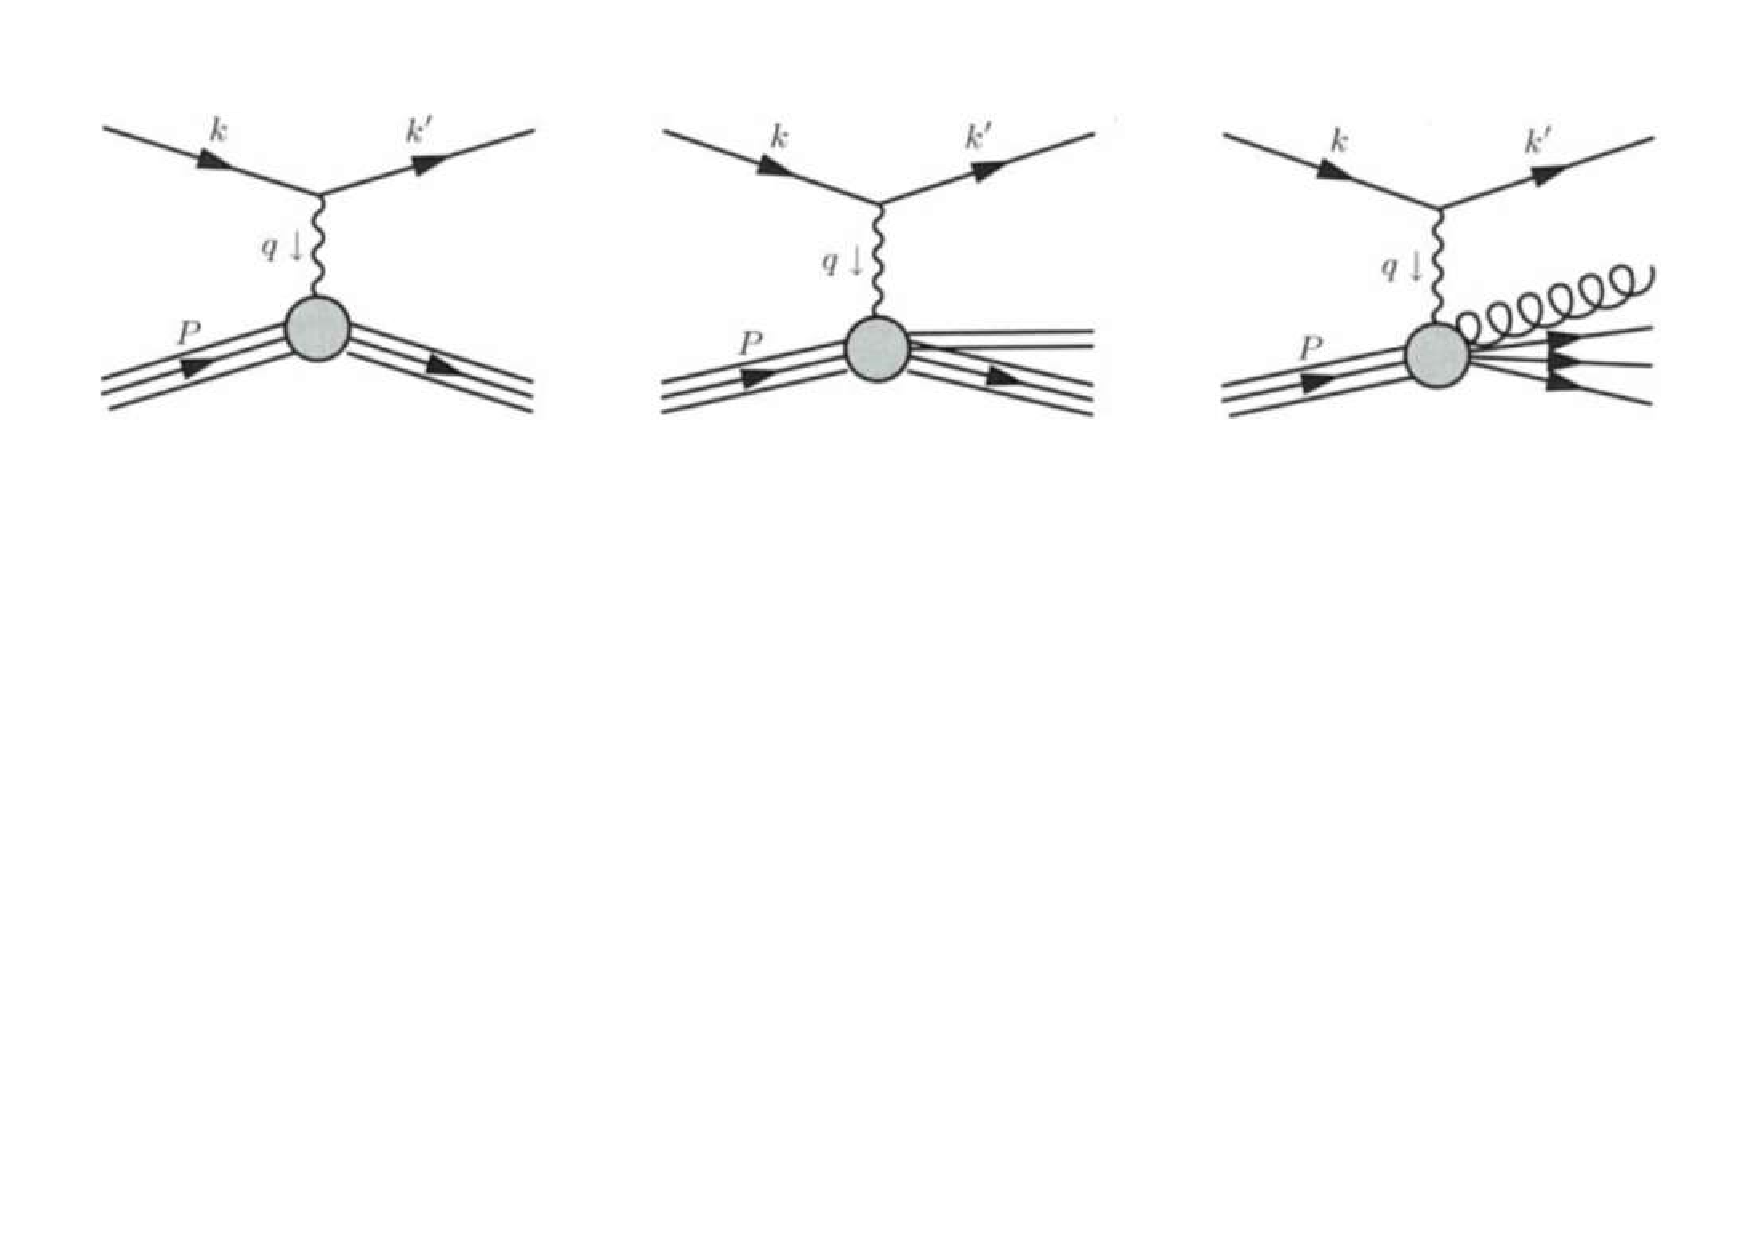
\includegraphics[scale=0.5]{DIS.pdf}
\caption{Elastic, inelastic and deep inelastic scattering \cite[pg 672]{Schwartz}}
\label{fig:DIS}
\end{center}
\end{figure}

In order to explain this, Bjorken and Feynman proposed the \emph{parton model} of hadron structure, which models hadrons as collections of collinearly moving \emph{partons}, i.e. quarks, anti-quarks and the bosons holding the hadron together \cite[pg 54]{PeskinSchroeder}.

\begin{figure}[h]
\begin{center}
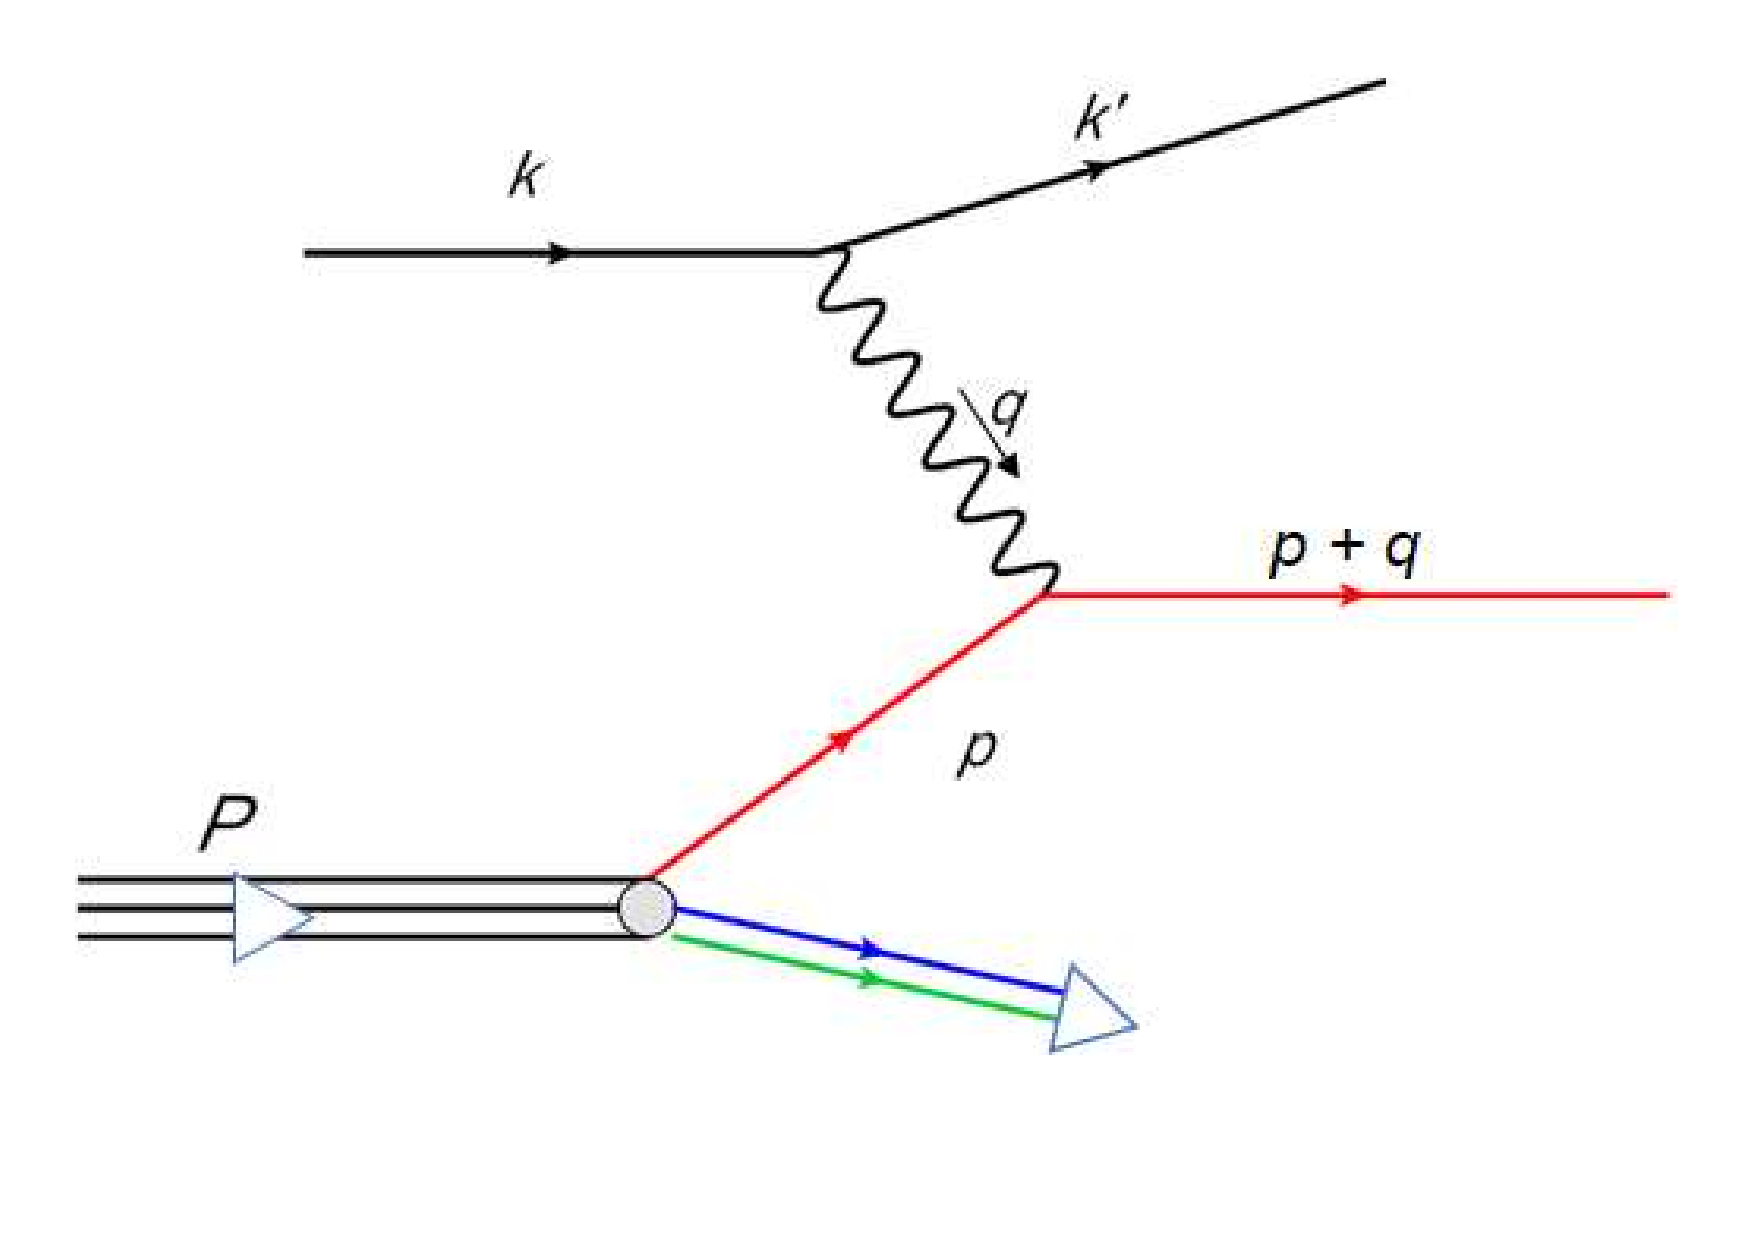
\includegraphics[scale=0.3]{Parton_Model.pdf}
\caption{The \emph{Parton model} of hadron structure \cite[pg 54]{Gardi:QCD}}
\label{fig:Parton_Model}
\end{center}
\end{figure}

Closely following the outline given in \cite[chapter 11]{Gardi:QCD} and \cite[chapter 14]{PeskinSchroeder}, we now outline the parton model for electron-proton scattering i.e.:
\begin{align}
e^{-} \lr{k} + p \lr{P} &\rightarrow e^{-} \lr{k'} + X
\end{align}
where $X$ is a final state consisting of a jet (i.e. multiple, unspecified) of hadrons. The \emph{kinematics} (energies of the particles concerned) are shown in Fig \ref{fig:Parton_Model}, where $p$ is the momentum of the struck quark and $p=\xi P$, where $\xi$ is the fraction ($0 \le \xi \le 1$) of hadron momentum $P$ carried by the scattering quark. The momentum is transferred by a (highly virtual) photon of momentum $q$.

Defining \cite[pg 54]{Gardi:QCD}:
\begin{align}
f_f \lr{\xi}\dd{\xi} \equiv &\textrm{ probability of finding a parton $f$ with momentum fraction $\xi$ inside the hadron}\\
\hat{\sigma} \equiv &\textrm{ partonic cross-section, i.e. } \hat{\sigma} \lr{ e^- \lr{k} + q \lr{ \xi P} \rightarrow e^- \lr{k'} + q}\\
\sigma \equiv &\textrm{ hadronic cross-section, i.e. } \sigma \lr{ e^- \lr{k} + p \lr{P} \rightarrow e^- \lr{k'} + X}
\end{align}
The importance of the parton model is that it allows us to compute the hadronic cross-section, $\sigma$, despite the inability to calculate them from first principles using QFT. We calculate the partonic cross-sections, $\hat{\sigma}$, from first principles using QFT, then sum over all possible parton types, and integrate over all possible momenta i.e.:
\begin{align}
\label{eq:DIS1} \sigma &= \int_0^1 \dd{\xi} \sum_f f_f \lr{\xi} \hat{\sigma}
\intertext{provided we know the PDF, $f_f \lr{\xi}$.}
\intertext{We will see below (\S \ref{sec:theory_Bjorken}) that (to first order) the structure of hadrons is independent of the energy scale, depending only on $\xi$. Thus, the PDF is essentially a probability distribution such that $f_f \lr{\xi} \dd{\xi}$ is the probability of finding a parton carrying momentum fraction $\xi$ in the narrow band $\dd{\xi}$, normalised so that:}
1 &= \int_0^1 f_f \lr{\xi} \dd{\xi}
\end{align}

\subsection{Useful kinematic variables in DIS}

Here, we define three commonly used DIS kinematic variables: $x$; $Q^2$; and $W^2$.

Assuming massless particles ($p^2 = k^2 = k'^2 = 0$), the Mandelstam invariants are:
\begin{align}
\hat{s} &= \lr{p + k}^2 = 2 p \cdot k > 0\\
\hat{t} &= \lr{k - k'}^2 = -2 k \cdot k' < 0\\
\hat{u} &= - \hat{s} - \hat{t}
\intertext{Conservation of momentum at the electron vertex gives $k = k' + q \implies \hat{t} = -q^2$, hence it is usual in DIS to define:}
\label{def:Q2} Q^2 &= -q^2 = - \hat{t} > 0
\intertext{i.e. $Q$ is the energy scale with which the electron probes the hadron's structure.}
\intertext{Considering the quark-photon vertex in Fig \ref{fig:Parton_Model}, to leading-order the final-state product is a single scattered quark which emerges on-shell. Again, considering massless particles, i.e.:}
\lr{p + q}^2 &= 0
\intertext{but $p = \xi P$ and $p^2=0$, so:}
2 \xi P \cdot q &= Q^2
\intertext{which is why it is usual to define the kinematic variable $x$:}
\label{def:x} x &= \frac{Q^2}{2 P \cdot q}
\intertext{where $x$ corresponds to the fraction of the hadron's momentum carried by the struck parton, i.e. $x = \xi$.}
\intertext{Another useful kinematic variable in DIS is $W^2$, defined \cite[pg 8]{Roberts} to be the square of the momentum of the final hadronic jet (the struck quark plus the rest of the shattered nucleon), i.e.:}
W^2 &= \lr{P + q}^2
\intertext{which for a nucleon of mass $M$ and using $2 P \cdot Q = \flatfrac{Q^2}{x}$ gives:}
\label{def:W2} W^2 &= \frac{Q^2 \lr{1 - x}}{x} + M^2
\end{align}

This derivation is to first-order, but the use of $Q^2$, $x$ and $W^2$ remain useful to all orders throughout DIS. The lowest energy scale we consider in this project is around $Q^2 = 5$ G eV$^2$, justifying the assumption of massless particles.

\subsection{Bjorken scaling and structure functions} \label{sec:theory_Bjorken}

To leading order, we compute the cross-section in Fig \ref{fig:Parton_Model}, $\hat{\sigma}$, obtaining:
\begin{align}
\dv{\hat{\sigma}}{\abs{\hat{t}}} &= \frac{1}{16 \hat{s}^2} \lr{\frac{1}{4} \sum_{\textrm{spins}} \abs{\mathcal{M}} ^2}\\
\label{eq:DIS2} &= \frac{2 \pi \alpha^2 Q_f^2}{\hat{s}^2} \lr{\frac{\hat{s}^2 + \hat{u}^2}{\hat{t}^2}}
\end{align}
where $Q_f$ is the electric charge of the quark, the strong coupling constant $\alpha = \flatfrac{e^2}{\lr{4 \pi}}$.

Inserting equation (\ref{eq:DIS2}) into equation (\ref{eq:DIS1}) we obtain the leading order result:
\begin{align}
\label{eq:theory_DIS3} \frac{\dd{\sigma}}{\dd{Q^2} \dx} &= \frac{2 \pi \alpha^2}{Q^4} \sum_f f_f \lr{x} Q_f^2 \lr{1 + \lr{ 1 - \frac{Q^2}{xs}}^2 }
\intertext{where as Peskin and Schroeder \cite[pg 478]{PeskinSchroeder} note, all of the kinematic dependence is contained in the factor:}
\label{eq:theory_BjorkenScaling} &\quad \frac{1 + \lr{ 1 - \frac{Q^2}{xs}}^2}{Q^4}
\end{align}
and the remaining kinematic dependence on $x$, once this factor is removed, is referred to as \emph{Bjorken scaling}. ``Bjorken scaling is, essentially, the statement that the structure of the proton looks the same to an electromagnetic probe no matter how hard the proton is struck'' \cite[pg 478]{PeskinSchroeder}.

Adding \emph{quantum chromodynamics} (QCD) corrections \cite[see][pp 557-8 for derivation]{PeskinSchroeder} and defining the kinematic variable:
\begin{align}
y &= \frac{2 P \cdot q}{2 P \cdot k}
\intertext{we obtain:}
\label{eq:DIS3} \frac{\dd{\sigma}}{\dd{Q^2} \dx} &= \frac{4 \pi \alpha^2}{x y Q^2} \lrb{ x y^2 F_1 \lr{x, Q^2}  + \lr{1 - y} F_2F_1 \lr{x, Q^2}}
\end{align}
where, $F_1\lr{x, Q^2}$ and $F_2\lr{x, Q^2}$ are referred to as structure functions and encapsulate our knowledge of the structure of hadrons (NB: the structure functions are different for each hadron). Although we can examine $F_1$ and $F_2$ analytically we cannot compute them, so we reconstruct them based on experimental data such as from DIS experiments. In practice, these structure functions are normally provided in the form of computer software, such as LHAPDF \cite{LHAPDF}, which were used in this project.

\subsection{Structure functions and PDFs} \label{sec:theory_structure_pdf}

At higher energy scales, \emph{Bjorken scaling violations} occur; i.e. the energy dependence of cross-sections is more complex than the factor in equation (\ref{eq:theory_BjorkenScaling}). Nevertheless, it is still true that there is an exact relationship between the evolution of structure functions from one energy scale to another, and the equation describing it is named the DGLAP (Dokshitzer, Gribov, Lipatov, Altarelli and Parisi) equation \cite[\S32.2, pg 677-81]{Schwartz}.

Accordingly, we expand our definition of PDFs to be functions of both momentum fraction and energy, i.e. $f_f \lr{x, Q^2}$. PDFs are are specific to the hadron they describe, and are normally named after the quarks ($u$, $d$, $c$, $s$, $t$ and $b$), anti-quarks ($\bar{u}$, $\bar{d}$, $\bar{c}$, $\bar{s}$, $\bar{t}$ and $\bar{b}$) and gluons ($g$) they represent. For example $u \lr{x, Q^2} \dx$ is the probability of finding an up quark with momentum-fraction between $x$ and $x + \dx$ when probed with an energy $Q^2$, and we have different specialisations of $u \lr{x, Q^2}$ for protons vs neutrons.

PDFs and structure functions are related \cite[pg 337]{BurgessMoore}:
\begin{align}
\label{eq:F_1_PDF} F_1 \lr{x, Q^2} &= \frac{1}{2} \sum_m \lrb{\frac{4}{9} \lr{u_m + \bar{u}_m} \lr{x, Q^2} + \frac{1}{9} \lr{d_m + \bar{d}_m} \lr{x, Q^2}}
\intertext{where the $m$ are the generations of matter.}
\intertext{Furthermore, the Callan-Gross relation tells us that the structure functions are not independent, but related:}
\label{eq:F_2_PDF} F_2 \lr{x, Q^2} &= 2 x F_1 \lr{x, Q^2}
\end{align}
at least to third order, where gluon interactions appear. This justifies the focus in this project on structure function $F_2$ at NNLO.

\subsection{Higher twist} \label{sec:theory_HT}

In the derivation of equation (\ref{eq:DIS3}), we find an Operator Product Expansion defining higher twist'', $T$, of the form (for full details of the operator product expansion, see Peskin and Schroeder \cite[pp 627-32]{PeskinSchroeder}):
\begin{align}
\int \dd[4]{x} &\exp^{\im q \cdot x} T \lr{\bar{\psi} \lr{x} \gamma^\mu \psi \lr{x} \bar{\psi} \lr{0} \gamma^\nu \psi \lr{0}}\\
&= - \im \bar{\psi} \lr{0} \lr{\gamma^\mu \im \partial^\nu + \gamma^\nu \im \partial^\mu - g^{\mu \nu} \slashed{q}}
\frac{1}{Q^2} \sum_{n=0}^\infty \lr{ \frac{2 \im q \cdot \partial}{Q^2} }^n \psi \lr{0}
%\\ &\quad + \textrm{higher twists}
\end{align}
What is important to note for this project is:
\begin{itemize}
\item This is an infinite series suppressed by an expansion term of $\order{\flatfrac{1}{Q^2}}$
\item In the high-momentum, low energy (i.e. high-$x$, low-$Q^2$) limit, the twist terms become infinite
\end{itemize}
i.e. we are unable to obtain a finite answer using this method in this regime. This is the infinity that was referred to in the introduction.

\subsection{Impact of higher twist on PDFs} \label{sec:theory_motivation}

Because of the problems computing higher twist, many PDF collaborations, including NNPDF, exclude experimental data in the high-$x$, low-$Q^2$ regime from their construction of PDFs \cite{NNPDF31}.

This provides the rationale for this project -- if we can find a theory-free, empirical model for higher twist, then it may be possible to include more data in the construction of PDFs, improving their accuracy at high-$x$ and low-$Q^2$, where they are currently poorly defined.

The intention is to follow the statistical methodology developed by NNPDF \cite{NNPDF:Reweight1} \cite{NNPDF:Reweight2} to assess the impact of a new higher twist model on the theoretical predictions embodied in PDFs. First, we will cover the necessary statistics, then return to higher twist and PDFs in \S \ref{sec:reweighting}.

\section{Statistics} \label{sec:theory_stats}

We will be processing data sets that are measurements of the structure function, $F_2$, together with statistical and systematic errors. The theory required to understand the statistical methods employed in this project is outlined below. As a computational project, the intention was to use established statistical techniques to obtain a result, rather than develop new statistical methods.

\subsection{Expectation values and variance}

For $N$ measurements of the same observable, $x_i$, we define the true mean, $\mu$, as the expected value of $x$, i.e. $\mu = \expval{x}$ where:
\begin{align}
\label{theory_mean1} \expval{x} &= \frac{1}{N} \sum_{i=1}^N x_i
\intertext{and the variance, $\sigma^2 = \expval{\lr{x - \expval{x}}^2}$, as:}
\label{theory_var1} \sigma^2 &= \frac{1}{N} \sum_{i=1}^N \lr{x_i -\mu}^2
\end{align}
both taken in the limit of an infinite number of observations, i.e. as $N \rightarrow \infty$ \cite[pg 12]{Lyons}.

For a real data set, where the true values of $\mu$ and $\sigma^2$ are unknown, the best estimate of the mean, $\bar{x}$, becomes \cite[pg 12]{Lyons}:
\begin{align}
\label{theory_mean2} \bar{x} &= \frac{1}{N} \sum_{i=1}^N x_i
\intertext{and the best estimate of the variance, $s^2$, becomes:}
s^2 &= \frac{1}{N - 1} \sum_{i=1}^N \lr{x_i -\mu}^2
\end{align}

However, unless $N$ is small, the difference between equations (\ref{theory_mean2}) and (\ref{theory_mean1}) is negligible. Given the size of the data sets in this project, we use equation (\ref{theory_mean1}) for variance, except as specifically noted.

\subsection{Combining errors}

In this project, we use the notation $\sigma = \sqrt{\sigma^2}$ to denote error $= \sqrt{\textrm{variance}}$ and all charts use $\sigma$ for error bars (unless explicitly stated otherwise).

\subsubsection{Adding errors}

For situations where we wish to combine two measurements, say $a = b - c$, with variances $\sigma_a^2$, $\sigma_b^2$ and $\sigma_c^2$ respectively, applying equation (\ref{theory_var1}) \cite[pg 23]{Lyons}:
\begin{align}
\sigma_a^2 &= \expval{\lr{b - c - \expval{b - c}}^2}\\
&= \expval{\lr{b - \expval{b}}^2} + \expval{\lr{c - \expval{c}}^2} - 2 \expval{\lr{b - \expval{b}} \lr{c - \expval{c}}}
\intertext{and for uncorrelated errors, the last term averages to zero yielding:}
\label{eq:theory_quad} \sigma_a^2 &= \sigma_b^2 + \sigma_c^2
\end{align}
Equation (\ref{eq:theory_quad}) is referred to as the addition of errors \emph{in quadrature}.

\subsubsection{Multiplying and dividing errors}

For a more complex case, where we define a function, $f \lr{x, y}$, where $x$ and $y$ have associated errors $\sigma_x^2$ and $\sigma_y^2$ such that:
\begin{align}
f &= x^a y^b, & \lr{a,b \in \mathbb{R}}
\intertext{we take the $\ln$ of both sides, then differentiate, obtaining:}
\frac{\delta f}{f} &= a \frac{\delta x}{x} + b \frac{\delta y}{y}
\intertext{and we add the errors in quadrature (equation \ref{eq:theory_quad}) obtaining:}
\label{eq:theory_combine_errors} \lr{\frac{\sigma_f}{f}}^2 &= a^2 \lr{\frac{\sigma_x}{x}}^2 + b^2 \lr{\frac{\sigma_y}{y}}^2
\end{align}
which for simple cases where $a,b = \pm 1$ is simply the statement that the \emph{relative error} in $f$ is obtained by adding the relative errors on $x$ and $y$ in quadrature \cite[pg 25]{Lyons}.

\subsection{Experimental error, covariance and correlation} \label{theory:covar}

This project uses experimental measurents of the structure function, $F_2$, for protons and neutrons from BCDMS \cite[Proton]{BCDMS:Proton} \cite[Deuteron]{BCDMS:Deuteron}, JLAB \cite{JLAB} and SLAC \cite{Whitlow}.

The data presented all consist of experimental measurements of $F_2\lr{x, Q^2}$ at various points in the $x$-$Q^2$ plane, and each measurement is stated together with associated statistical error, $\sigma_{\textrm{stat}}$, and systematic error, $\sigma_{\textrm{sys}}$.

In addition to the statistical and systematic errors published, each of the papers describes various sources of normalisation error, $\sigma_N$, arising due to the experimental setup and typically depending on targets, beam energies and other factors in the experimental setup. We defer detailed discussion of normalisation error for each experiment to \S \ref{sec:design_normalisation}. For the purposes of this chapter, however, we define normalisation error, $\sigma_N^2 \lr{S_i, S_j}$, as a function of the experimental data sets ($S_i$ and $S_j$) to which any two measurements belong.

The \emph{covariance}, $\sigma_{ij}$, between any two data points $x_i$ and $x_j$ defined as \cite[pg 26]{James}:
\begin{align}
\label{eq:theory_covar} \sigma_{ij} &= \expval{x_i - \expval{x_i}} \expval{x_j - \expval{x_j}}
\intertext{and we construct the \emph{experimental covariance matrix}, $\sigma_{ij}$:}
\label{eq:theory_exp_covar} \sigma_{ij} &= \delta_{ij} \lr{\sigma_{\textrm{stat},i} \sigma_{\textrm{stat},j}}
+ \sigma_{\textrm{sys},i} \sigma_{\textrm{sys},j}
+ \sigma_N^2 \lr{S_i, S_j}
\intertext{which we can then normalise to construct the \emph{correlation matrix}, $\rho_{ij}$:}
\label{eq:theory_correl} \rho_{ij} &= \frac{\sigma_{ij}}{\sqrt{\sigma_i \sigma_j}}
\end{align}
with every element between $1$ (perfectly positively correlated), $0$ (uncorrelated) and $-1$ (perfectly anti-correlated).

\subsection{$\chi^2$ hypothesis testing}

In order to test the hypothesis that a series of $N$ experimental measurements of data points $D_i$ (i.e. $N$ \emph{degrees of freedom}) are consistent with corresponding theoretical predictions $T_i$, we define the $\chi^2$ statistic using the \emph{covariance form} of $x_i$ as \cite[pg 69]{James}:
\begin{align}
\label{theory_chisq} \chi^2 &= \sum_{i,j=1}^N \lr{D_i - T_i} \sigma_{ij}^{-1} \lr{D_j - T_j}
\intertext{where $\sigma_{ij}^{-1}$ is the inverse of the covariance matrix.}
\intertext{This has a $\chi^2$ distribution \cite[pg 69]{James}, so if the hypothesis is correct, the expectation value of $\chi^2$ is the number of degrees of freedom, i.e.:}
\expval{\chi^2} &= N
\intertext{We normalise these results by defining the reduced chi-squared, $\chi_\nu^2 = \flatfrac{\chi^2}{N}$:}
\label{theory_chisq_r} \chi_\nu^2 &= \frac{1}{N} \sum_{i,j=1}^N \lr{D_i - T_i} \sigma_{ij}^{-1} \lr{D_j - T_j}
\intertext{which has an expectation value, if the hypothesis is true, of:}
\expval{\chi_\nu^2} &= 1
\end{align}

As an estimate of the goodness of fit, the $\chi_\nu^2$ statistic allows different theoretical models to be compared with a data set, with the model with the lower $\chi_\nu^2$ being a better fit.

\subsection{Monte Carlo representations and re-weighting} \label{sec:reweighting}

Monte Carlo representations of theoretical predictions, $t$, consist of an ensemble of replicas of $t$, constructed in such a way that the mean and variance of $t$ can be determined by a simple average over the replicas. This simplifies theoretical error propagation, especially for complex, multi-dimensional predictions such as those embodied in PDFs \cite[pg 4]{d'Agostini}, which is why software such as LHAPDF \cite{LHAPDF} presents them as Monte Carlo replicas.

In addition to the PDFs used in this project, the higher twist model we develop is also held in Monte Carlo representation. We do this so we can apply the reweighting technique described here in order to optimise it (we discuss the model itself in \S \ref{sec:design_model_build}).

The NNPDF collaboration developed \cite{NNPDF:Reweight1} \cite{NNPDF:Reweight2} methods for optimising Monte Carlo representations of theoretical predictions based on use of the $\chi^2$ statistic. These methods were developed for application to PDFs, but can be used more widely. In this project we use this technique to:
\begin{enumerate}
\item Optimise our higher twist model using data not used in the construction of NNPDF 3.1 replicas \cite{NNPDF31}
\item Assess the impact the higher twist model would have on the NNPDF 3.1 PDF replicas.
\end{enumerate}

We rely on the same result in both cases, the \emph{reweighting formula} \cite[equation 9]{NNPDF:Reweight1}, which says that for a Monte Carlo representation consisting of $N$ replicas of theoretical predictions $T_i$, if we use equation (\ref{theory_chisq}) to calculate the $\chi^2$ statistic for the $k$-th replica, $\chi_k^2$, then we can assign a weight to each replica, $w_k$:
\begin{align}
\label{eq:theory_reweight} w_k &= \frac{\lr{\chi_k^2}^{\flatfrac{\lr{n-1}}{2}} \exp^{- \flatfrac{\chi_k^2}{2}}}{\frac{1}{N} \sum_{k = 1}^N \lr{\chi_k^2}^{\flatfrac{\lr{n-1}}{2}} \exp^{- \flatfrac{\chi_k^2}{2}}}
\intertext{where ``$\flatfrac{w_k}{N}$ is the probability of each replica given the $\chi^2$ to the new data''\cite[\S 2.1]{NNPDF:Reweight1}.}
\intertext{Furthermore, the effective number of replicas of the reweighted set, $N_\textrm{eff}$ \cite[equation 9]{NNPDF:Reweight1} $\lr{0 < N_\textrm{eff} < N}$ is calculated:}
\label{eq:theory_Neff} N_\textrm{eff} &= \exp{\frac{1}{N} \sum_{k=1}^N w_k \ln \lr{\frac{N}{w_k}}}
\end{align}

\subsection{Avoiding d'Agostini bias in PDF reweighting} \label{theory:d'Agostini}

The NNPDF collaboration noted \cite[\S6 and \S7]{d'Agostini} that in the context of PDF reweighting, under-estimation of errors in the $\chi^2$ statistic can occur when using data with normalisation errors spanning multiple experiments, as is the case for this analysis. They recommended that, to avoid `d'Agostini bias', any normalisation uncertainties used in the construction of the covariance matrices be scaled, not by the experimentally measured data point but by the central replica (i.e. mean) theoretical prediction. Accordingly, this recommendation is followed in the construction of the normalisation error component of the experimental covariance matrices.



%%%%%%%%%%%%%%%%%%%%%%%
\chapter{Project design}

\section{Overview}

\subsection{Aims} \label{design:aims}

Motivated by the considerations outlined in \S \ref{sec:theory_motivation}, the aims of this project were to:
\begin{itemize}
\item Construct an empirical higher twist model, using high-$x$, low-$Q^2$ scattering data
\item Determine whether the model improved the $\chi^2$ fit of PDFs to the data
\item Qualitatively assess the impact of the higher twist model on PDF predictions.
\end{itemize}

\subsection{Scope} \label{design:scope}

Being an MSc project, we made the following decisions to constrain our scope:

\begin{enumerate}
\item The higher twist model was a simple, Monte Carlo ensemble of replicas, with weights determined using the techniques outlined in \S \ref{sec:reweighting}
\item Impact assessment on PDFs was restricted to NNPDF 3.1 \cite{NNPDF31}
\item Analysis was restricted to variable kinematic cuts in one dimension only, $W^2$.
\end{enumerate}

\subsection{Custom software}

I wrote 7380 lines of c++ source code, unaided and from scratch for this project. The software is designed to process proton and deuteron data either independently or combined, because a-priori we did not know which would generate a successful model.

We target Linux in order to make use of the following freely available scientific libraries:
\begin{itemize}
\item \emph{APFEL} \cite{APFEL}: DGLAP evolution of $F_2$ structure function predictions to required energy scales
\item \emph{LHAPDF} \cite{LHAPDF}: raw PDF provision (for consumption via APFEL)
\item \emph{CERN ROOT} \cite{ROOT}: matrix inversion and automated graphing
\end{itemize}
Though not a goal of the original design, given the volume of data and the number of graphs required, the decision was taken during the project to automate all charts using ROOT. Note that all statistics presented in this report are calculated within the code developed for this project (not ROOT).

The following sections outline:
\begin{itemize}
\item Experimental data sets used
\item Construction of the experimental covariance matrices
\item Higher twist model
\item Data flow, i.e. how the software was used for analysis.
\end{itemize}

\section{Rationale for choice of data sets}

High-$x$, low-$Q^2$ experimental measurements of $F_2$ were required to:
\begin{table}[H]
\begin{center}
\begin{tabular}{|l|l|}
\hline
\textbf{Reason data required} & \textbf{Data needed}\\
\hline
Build higher twist model & Additional (not included in NNPDF 3.1)\\
\hline
Validate higher twist model & Included in NNPDF 3.1 $+$ additional\\
\hline
\end{tabular}
\caption{Data sets required for analysis}
\label{tb:design_datasets_required}
\end{center}
\end{table}

Data sets used for analysis, and whether data are included in / additional to NNPDF:
\begin{table}[H]
\begin{center}
\begin{tabular}{|c|p{8cm}|c|c|}
\hline
\multirow{2}{*}{\textbf{Data set}} & \multirow{2}{*}{\textbf{Rationale for inclusion of data set}} & \multicolumn{2}{c|}{\textbf{NNPDF 3.1}}\\
\cline{3-4}
&& \textbf{Included} & \textbf{Additional}\\
\hline
BCDMS \cite{BCDMS:Deuteron} \cite{BCDMS:Proton} & Previous analyses \cite{Milsztajn:Data} show both data sets & \checkmark & \checkmark\\
\cline{1-1} \cline{3-4}
SLAC \cite{Whitlow} & compatible, despite larger errors in SLAC & \checkmark & \checkmark\\
\hline
\multirow{2}{*}{JLAB \cite{JLAB}} & Gives at least one high-precision $F_2$ data set not used in NNPDF 3.1 construction&& \multirow{2}{*}{\checkmark}\\
\hline
\end{tabular}
\caption{Data sets chosen for analysis}
\label{tb:design_datasets_chosen}
\end{center}
\end{table}

The kinematics of the combined dataset\footnote{Using the NNPDF version of the SLAC dataset (see \S \ref{sec:SLAC_reanalyzed})}$^,$\footnote{A kinematic cut at $W^2\ge3.5$ GeV$^2$ was inadvertently applied to the NNPDF version of the SLAC dataset; however as we shall see in Ch. \ref{ch:results}, our algorithms apply kinematic cuts to the data -- the lowest being at $W^2\ge5$ GeV$^2$ -- so the missing 17 SLAC data points have no impact.} are displayed graphically in figs \ref{fig:design_kinematics_PAN} and \ref{fig:design_kinematics_NNPDF_PHN}.

\begin{figure}[h]
\begin{center}
\includegraphics[scale=0.89]{Graphs/DataSet_NNPDF_All.pdf}
\caption{Kinematics of the datasets used in this project}
\label{fig:design_kinematics_PAN}
\end{center}
\end{figure}

NNPDF 3.1 construction used data surviving kinematic cuts at \cite[Table 2.4, pg 9]{NNPDF31}:
\begin{align}
W^2 &\ge 12.5 \textrm{ GeV}^2\\
Q^2 &\ge 3.5 \textrm{ GeV}^2
\end{align}

Accordingly, we split our data set into high (data points above the NNPDF 3.1 cutoff, table \ref{tb:Kinematics_High}) and low (data points below the cutoff, table \ref{tb:Kinematics_Low}).
\begin{figure}[h]
\begin{center}
\includegraphics[scale=0.42]{Graphs/DataSet_NNPDF_High.pdf}\includegraphics[scale=0.42]{Graphs/DataSet_NNPDF_Low.pdf}
\caption{Kinematics of the high / low datasets (above / below NNPDF 3.1 cutoff)}
\label{fig:design_kinematics_NNPDF_PHN} \label{fig:design_kinematics_NNPDF_PLN}
\end{center}
\end{figure}

\begin{table}[h]
\begin{center}
\begin{tabular}{|c|c|c|c|c|}
\hline
Data set & $N_{\textrm{Proton}}$ & $N_{\textrm{Deuteron}}$ & $W^2$ / GeV$^2$ & $Q^2$ / GeV$^2$\\
\hline
BCDMS & $333$ & $248$ & $ 13.2 \le W^2 \le 350$ & $ 7.5 \le Q^2 \le 230$ \\
SLAC (NNPDF) & $33$ & $34$ & $ 12.5 \le W^2 \le 30.7$ & $ 3.5 \le Q^2 \le 19.5$ \\
SLAC (reanalyzed) & $90$ & $90$ & $ 12.5 \le W^2 \le 30.7$ & $ 3.5 \le Q^2 \le 21.4$ \\
\hline
\end{tabular}
\caption{High (above NNPDF 3.1 cutoff) data set kinematics}
\label{tb:Kinematics_High}
\end{center}
\end{table}

\begin{table}[h]
\begin{center}
\begin{tabular}{|c|c|c|c|c|}
\hline
Data set & $N_{\textrm{Proton}}$ & $N_{\textrm{Deuteron}}$ & $W^2$ / GeV$^2$ & $Q^2$ / GeV$^2$\\
\hline
BCDMS & $18$ & $6$ & $ 7.1 \le W^2 \le 12.5$ & $ 11.7 \le Q^2 \le 37.5$ \\
JLAB & $261$ & $265$ & $ 0.25 \le W^2 \le 4.25$ & $ 3.5 \le Q^2 \le 7.4$ \\
SLAC (NNPDF) & $161$ & $160$ & $ 1.6 \le W^2 \le 30.1$ & $ 1 \le Q^2 \le 29.2$ \\
SLAC (reanalyzed) & $545$ & $575$ & $ 2.1 \le W^2 \le 26.7$ & $ 1 \le Q^2 \le 30.3$ \\
\hline
\end{tabular}
\caption{Low (below NNPDF 3.1 cutoff) data set kinematics}
\label{tb:Kinematics_Low}
\end{center}
\end{table}

\subsection{Multiple versions of the SLAC dataset} \label{sec:SLAC_reanalyzed}

Please note that two versions of the SLAC dataset were used, referred to as:
\begin{itemize}
\item NNPDF: the original published SLAC dataset as used by NNPDF\\
\item Reanalyzed \cite{Whitlow}: re-procesed data, binned more finely in $x$.
\end{itemize}

The SLAC (NNPDF) dataset was used to generate NNPDF 3.1 \cite{NNPDF31}, making this version necessary for this analysis. This dataset was provided by Prof Ball's PhD student, \mbox{Rosalyn} \mbox{Pearson} (both members of the NNPDF collaboration). This is the version of the SLAC data set used in this analysis unless explicitly stated otherwise.

The SLAC (reanalyzed) dataset is the publicly available version of the same dataset. It contains more data points, as it is more finely binned in $x$ (figs \ref{fig:design_kinematics_PAr} and \ref{fig:design_kinematics_PHr}).
\begin{figure}[h]
\begin{center}
\includegraphics[scale=0.89]{Graphs/DataSet_reanalyzed_All.pdf}
\caption{Kinematics using the reanalyzed SLAC dataset}
\label{fig:design_kinematics_PAr}
\end{center}
\end{figure}

\begin{figure}[h]
\begin{center}
\includegraphics[scale=0.42]{Graphs/DataSet_reanalyzed_High.pdf}\includegraphics[scale=0.42]{Graphs/DataSet_reanalyzed_Low.pdf}
\caption{Kinematics using the reanalyzed SLAC dataset (high / low)}
\label{fig:design_kinematics_PHr} \label{fig:design_kinematics_PLr}
\end{center}
\end{figure}

\subsection{Construction of experimental covariance matrices} \label{sec:design_normalisation}

The experimental covariance matrices (\S \ref{theory:covar}) are constructed (equation \ref{eq:theory_exp_covar}) using the statistical error, $\sigma_{\textrm{stat}}$, and systematic error, $\sigma_{\textrm{sys}}$, for each data point:
\begin{align}
 \sigma_{ij} &= \delta_{ij} \lr{\sigma_{\textrm{stat},i} \sigma_{\textrm{stat},j}}
+ \sigma_{\textrm{sys},i} \sigma_{\textrm{sys},j}
+ \sigma_N^2 \lr{S_i, S_j}
\end{align}

However, overall normalisation errors, $\sigma_N$, are not available as part of the data, but are described in the papers associated with each experiment. First, we provide an overview of the code developed to construct the experimental covariance matrices based on the descriptions in each paper, then detail the errors used for each experiment, with references to the appropriate paper. Conveniently, the data files used each have a header containing a reference to the paper describing the experiment.

For each of our datasets, normalisation errors are quoted as relative errors. In some cases there are multiple sources of normalisation error quoted, so we add the error sources in quadrature per equation (\ref{eq:theory_quad}). The total normalisation errors are then scaled, not by the data points for $F_2$ but rather by the central replica prediction for $F_2$, in order to avoid d'Agostini bias as outlined in \S \ref{theory:d'Agostini}.

Code listings for covariance element construction are given in appendix \ref{code:covar} and sample data file headers are listed in appendix \ref{data:header}.

\subsubsection{BCDMS}

Relative normalisation error, $\sigma_N$, for BCDMS \cite[pg 486]{BCDMS:Proton} \cite[pg 594-5]{BCDMS:Deuteron} \cite[pg 5]{Forte:2002fg} is:
\begin{equation}
\sigma_N^2 = \sigma_{N_a}^2 + \sigma_{N_t}^2 + \sigma_{N_b}^2
\end{equation}
where symbols are defined in table \ref{tb:BCDMS_Error_Sources} and take the values shown in table \ref{tb:BCDMS_Error_Values}.

\begin{table}[h]
\begin{center}
\begin{tabular}{|c|p{8.5cm}|c|}
\hline
Symbol & Description & Rel/Abs\\
\hline
$\sigma_{N_a}$ & Global (absolute cross-section) normalisation & Relative\\
$\sigma_{N_t}$ & Relative normalisation between targets & Relative\\
$\sigma_{N_b}$ & Relative normalisation between beam energies & Relative\\
\hline
\end{tabular}
\caption{BCDMS normalisation error sources}
\label{tb:BCDMS_Error_Sources}
\end{center}
\end{table}

Values for each error type and the conditions under which they apply:
\begin{table}[h]
\begin{center}
\begin{tabular}{|c|c|c|}
\hline
Symbol & Error & Condition\\
\hline
$\sigma_{N_a}$ & 3\% & all \\
\hline
\multirow{2}{*}{$\sigma_{N_t}$} & 0\% & same target \\
\cline{2-3}
& 2\% & different target\\
\hline
\multirow{4}{*}{$\sigma_{N_b}$} & 0\% & same beam energy or different target\\
\cline{2-3}
& 1\% & proton $-$ proton (all energies) \\
\cline{2-3}
& 1\% & deuteron (120GeV) $-$ deuteron (200 GeV) \\
\cline{2-3}
& 1.5\% & deuteron $-$ deuteron (other energies) \\
\hline
\end{tabular}
\caption{BCDMS normalisation error values}
\label{tb:BCDMS_Error_Values}
\end{center}
\end{table}

\subsubsection{JLAB}

Relative normalisation error, $\sigma_N$, for JLAB \cite[pg 486]{JLAB} is constant:
\begin{equation}
\sigma_N = 1.75 \textrm{ \%}
\end{equation}

\subsubsection{SLAC}

Relative normalisation error, $\sigma_N$, for SLAC \cite[pg 476]{Whitlow} is:
\begin{equation}
\sigma_N^2 = \sigma_{N_a}^2 + \sigma_{N_t}^2
\end{equation}
where symbols are defined in table \ref{tb:BCDMS_Error_Sources} and take the values shown in table \ref{tb:SLAC_Error_Values}.
\begin{table}[H]
\begin{center}
\begin{tabular}{|c|c|c|}
\hline
Symbol & Error & Condition\\
\hline
\multirow{2}{*}{$\sigma_{N_a}$} & 2.1\% & proton \\
\cline{2-3}
& 1.7\% & deuteron \\
\hline
$\sigma_{N_t}$ & 1.1\% & different targets \\
\hline
\end{tabular}
\caption{SLAC normalisation error}
\label{tb:SLAC_Error_Values}
\end{center}
\end{table}

\section{Data preparation}

Conceptually, the first phase of data processing was simple:
\begin{itemize}
\item A hierarchy of data types was developed to represent the data points from each data set, with the base class (see appendix \ref{code:DataNode}) containing the data members parsed or calculated from the input file.
\item To each data point we then added the full Monte Carlo set of NNPDF 3.1 theoretical predictions for $F_2 \lr{x, Q^2}$ using APFEL \cite{APFEL} and calculated to NNLO\footnote{Parameters used for APFEL are listed in appendix \ref{APFEL:Params}}
\item We then split each data set into ``high'' and ``low'' halves depending on whether the data point was included or excluded in NNPDF replica generation respectively.
\end{itemize}

Note: despite the conceptual simplicity of the task, we faced two large challenges:
\begin{itemize}
\item The APFEL DIS code had been re-written and did not match the documentation available in the paper \cite{APFEL}
\item PDF evolution took close to 36 hours for each of the data sets, necessitating the writing of extra code to cache the data sets.
\end{itemize}



\section{Software mode 1: build higher twist model} \label{sec:design_model_build}

To create a higher twist model we specified:
\begin{itemize}
\item The data set against which to perform the fit, where the data set must not have been used in NNPDF 3.1 generation\footnote{We define the terms \emph{low} and \emph{high}, in reference to data sets below and above the NNPDF 3.1 kinematic cuts respectively}
\item Which of the simple mathematical models to use (equations \ref{eq:model0}, \ref{eq:model1} or \ref{eq:model2})
\item Parameters (starting value, final value and number of steps)
\item Multiplicative (eq \ref{eq:multiplicative}) or additive (eq \ref{eq:additive}) mode
\item The range of cuts in $W^2$ (plus a fixed cut at $Q^2 \ge 1$).
\end{itemize}

The program ran in a loop, where for each cut:
\begin{itemize}
\item One replica of the model was created for every combination of parameters (usually 10,000 total)
\item The procedure outlined in \S \ref{sec:reweighting} was followed, using equation (\ref{eq:theory_reweight}) to generate weights, $w_k$, for every replica
\item The generated model was saved (as an input to later runs)
\item Data files and graphs were generated to summarise the results of the reweighting:
    \begin{itemize}
    \item Histograms of the parameter weights to aid model refinement
    \item $\chi_\nu^2$ before and after the fit (\S \ref{sec:design_chi_squared}, below)
    \item Number of effective replicas (equation \ref{eq:theory_Neff}) in the resulting model
    \item Summaries showing the $\chi_\nu^2$ statistic trends across the kinematic cuts specified.
    \end{itemize}
\end{itemize}

\subsection{Mathematical models}

The models were designed with these principles in mind:
\begin{itemize}
\item We wished to avoid building theoretical considerations into the raw model, relying instead on a weighted fit of the model to the data (\S \ref{sec:reweighting})
\item We needed a non-trivial model with as few parameters as possible in order to be able to execute the model on a laptop in a reasonable time
\item The $x$ and $\lr{1 - x}$ terms ensures the higher twist is small for $x=0$ and $x=1$
\item The $\lr{1 + d x}$ term allows the model to change sign.
\end{itemize}

The available mathematical models (see appendix \ref{code:Models} for code) consist of three raw models, $R_n \lr{x, Q^2, \vb{k}}$, (where $\vb{k} = \lr{a, b, c, d}$ is the $k$-th replica parameter vector):
\begin{align}
\label{eq:model0} R_0 \lr{x, Q^2, \vb{k}} &= c x^a \lr{1 - x}^b + \frac{d}{Q^2}\\
\label{eq:model1} R_1 \lr{x, Q^2, \vb{k}} &= c x^a \lr{1 - x}^b \lr{1 + d x}\\
\label{eq:model2} R_2 \lr{x, Q^2, \vb{k}} &= c x^a \lr{1 + b x} + \frac{d}{Q^2}
\intertext{Each model can be run in either additive mode where the contribution to the higher twist from replica $k$ is:}
\label{eq:additive} \delta F_2^{\textrm{HT},k} \lr{x, Q^2} &= \frac{R_n \lr{x, Q^2, \vb{k}}}{Q^2}
\intertext{or multiplicative mode where:}
\label{eq:multiplicative} \delta F_2^{\textrm{HT},k} \lr{x, Q^2} &= \frac{R_n \lr{x, Q^2, \vb{k}} F_2\lr{x, Q^2}}{Q^2}
\intertext{We calculate the contribution to $F_2$ from the entire set of $N$ model replicas, $\delta F_2^\textrm{HT} \lr{x, Q^2}$:}
\delta F_2^\textrm{HT} \lr{x, Q^2} & = \frac{1}{N} \sum_{k = 1}^N w_k \delta F_2^{\textrm{HT},k} \lr{x, Q^2}
\intertext{so that the prediction for $F_2$ including the higher twist, $F_2^\textrm{HT}$, is:}
\label{eq:f2_ht_mean} F_2^\textrm{HT} \lr{x, Q^2} &= F_2^\textrm{LT} \lr{x, Q^2} + \delta F_2^\textrm{HT} \lr{x, Q^2}
\end{align}
where: $F_2^\textrm{LT} \lr{x, Q^2}$ is the \emph{leading twist}, for which we use the NNPDF 3.1 prediction.

\subsection{Comparing $\chi_\nu^2$} \label{sec:design_chi_squared}

Equations (\ref{eq:additive}) and (\ref{eq:multiplicative}) were designed such that the \emph{higher twist covariance matrix} for our data set is also, using equation (\ref{eq:f2_ht_mean}), the \emph{theory covariance matrix}, which we calculate using equation (\ref{eq:theory_covar}):
\begin{align}
\label{eq:design_theory_covar} S_{ij} &= \frac{1}{N} \sum_{k = 1}^N w_k \lr{\delta F_2^{\textrm{HT},k} \lr{x_i, Q_i^2} - \delta F_2^\textrm{HT} \lr{x_i, Q_i^2}} \lr{\delta F_2^{\textrm{HT},k} \lr{x_j, Q_j^2} - \delta F_2^\textrm{HT} \lr{x_j, Q_j^2}}
\end{align}
It will be useful later to normalise $S_{ij}$ by defining the \emph{theory correlation matrix}, $\rho_{ij}$:
\begin{align}
\rho_{ij} &= \frac{S_{ij}}{\sqrt{S_{ii} S_{jj}}}
\end{align}

We then computed $\chi_\nu^2$, i.e. the fit for NNPDF 3.1 without our higher twist model, to the $N_{\textrm{dat}}$ data points, $D_i$, using equation (\ref{theory_chisq_r}) with $T_i= F_2 \lr{x_i, Q_i^2}$ and the experimental covariance matrix $\sigma_{ij}$, i.e.:
\begin{align}
\label{eq:design_chi} \chi_\nu^2 &= \frac{1}{N_{\textrm{dat}}} \sum_{i,j=1}^{N_{\textrm{dat}}} \lrc{D_i - F_2^\textrm{LT} \lr{x_i, Q_i^2}} \sigma_{ij}^{-1} \lrc{D_j - F_2^\textrm{LT} \lr{x_j, Q_j^2}}
\intertext{and we computed $\chi_{\nu,\textrm{HT}}^2$ of the fit with the higher twist model:}
\label{eq:design_chi_HT} \chi_{\nu,\textrm{HT}}^2 &= \frac{1}{N_{\textrm{dat}}} \sum_{i,j=1}^{N_{\textrm{dat}}} \lr{D_i - F_2^{\textrm{HT}} \lr{x_i, Q_i^2}} \lr{\sigma_{ij} + S_{ij}}^{-1} \lr{D_j - F_2^{\textrm{HT}} \lr{x_j, Q_j^2}}
\end{align}
Comparing these statistics computed using the data the models were constructed with yields:
\begin{align}
\chi_{\nu,\textrm{HT}}^2 &< \chi_\nu^2
\end{align}
except for cases where there were not enough data points to construct a useful model.

Defining $\chi_{\nu,\textrm{NNPDF}}^2$ as the statistic for the published value of NNPDF 3.1, if:
\begin{align}
\chi_{\nu,\textrm{HT}}^2 &< \chi_{\nu,\textrm{NNPDF}}^2
\end{align}
then we would expect the model to improve the fit over NNPDF 3.1, so we progressed to the model validation stage.

\section{Software mode 2: validate higher twist model} \label{sec:design_model_validate}

Specifying a pre-built model caused the program to validate the pre-built model against the chosen datasets, usually data used in NNPDF 3.1 construction, optionally including additional data. When multiple kinematic cuts were specified, we could either:
\begin{itemize}
\item Run models created at various kinematic cuts against the larger data set at corresponding kinematic cuts
\item Choose a single ``optimal'' model to validate at each of the specified kinematic cuts.
\end{itemize}
For each cut, the code:
\begin{itemize}
\item Applied the reweighting procedure (\S \ref{sec:reweighting}) to the PDF, generating weights $v_p$ for each of the $n$ PDF replicas (equation \ref{eq:theory_reweight}), and the number of effective PDF replicas, $N_\textrm{eff,PDF}$ (equation \ref{eq:theory_Neff})
\item The $\chi_\nu^2$ statistic we would expect from an improved NNPDF replica set containing $n$ replicas that incorporated the higher twist model:
\end{itemize}
\begin{equation}
\label{eq:chi_nu_HT_reweight} \chi_{\nu,\textrm{HT}}^{2,\textrm{r}} = \expval{\chi_{\nu,\textrm{HT}}^2} = \frac{1}{n} \sum_{p=1}^n v_p \chi_{\nu,\textrm{HT}}^2
\end{equation}
\begin{itemize}
\item Generated the same data and charts as produced when creating a model
\item The relationship between the structure functions and individual PDFs (equations \ref{eq:F_1_PDF} and \ref{eq:F_2_PDF}) allows estimation of the PDF predictions including a higher twist, $f_f^{\textrm{HT}}$, for $u$, $d$, $\bar{u}$, $\bar{d}$ and $g$ using:
\end{itemize}
\begin{align}
\label{eq:pdf_pred} f_f^{\textrm{HT}} \lr{x, Q^2} &= \frac{1}{n} \sum_{p=1}^n v_p f_f \lr{x, Q^2}
\end{align}

For any models where:
\begin{align}
\chi_{\nu,\textrm{HT}}^{2,r} &< \chi_{\nu,\textrm{NNPDF}}^2
\end{align}
then a new version of NNPDF, including the higher twist model, is expected to be a better fit to the data than NNPDF 3.1.



%%%%%%%%%%%%%%%%%%%%%%%
\chapter{Results and analysis} \label{ch:results}

For reference, we ran the software in mode 1 (\S \ref{sec:design_model_build}) using the high dataset and $W^2 \ge 12.5$ GeV$^2$ -- i.e. the data used in the construction of NNPDF 3.1 -- to calculate the reference statistic for the NNPDF 3.1 fit\footnote{More detailed checks are outlined in appendix \ref{code:covar}}, obtaining the same value for the proton and the deuteron:
\begin{align}
\label{eq:chisq_NNPDF} \chi_{\nu,\textrm{NNPDF}}^2 = 1.28
\end{align}

\section{Features of the higher twist model}

\subsection{Proton + deuteron models could not be generated} \label{sec_results_combined}

Combined models, using target data for both the proton and deuteron, were tested. However, the number of effective replicas of the resulting models were too low (less than 10\% of the starting number) to be useful. This was the expected result, which we attributed to the fact (as outlined near equation \ref{eq:DIS3}) that the structure functions differ for protons and deuterons.

\subsection{Separate models created for proton and deuteron} \label{sec_results_create}

Individual higher twist models for each of the proton and deuteron were constructed, following the procedure outlined in \S \ref{sec:design_model_build}, using the low data set, i.e. data not used to construct NNPDF 3.1. We repeated the model build phase multiple times for each model, tuning the model parameters until the number of effective replicas was maximised.

Best results were obtained using model 1 (equation \ref{eq:model1}) in additive mode. One Monte Carlo replica was constructed for every combination of parameters, $a$, $b$, $c$ and $d$. We show the starting value, increment (step) and number of steps (count) for each parameter:
\begin{table}[H]
\begin{center}
\begin{tabular}{|c|cccc|cccc|}
\hline
Parameter &\multicolumn{4}{c|}{Proton model}&\multicolumn{4}{c|}{Deuteron model}\\
\hline
Model 1, + & Min & Step & Max & Count & Min & Step & Max & Count\\
\hline
$a$ & $0.7$ & $0.0\dot{3}$ & $1$ & 10       & $0.85$ & $0.01\dot{6}$ & $1$ & 10\\
$b$ & $0.6$ & $0.1\dot{8}$ & $2.3$ & 10    & $0.8$ & $0.\dot{1}$ & $1.8$ & 10\\
$c$ & $-0.6$ & $0.0\dot{4}$ & $-0.2$ & 10  & $-0.5$ & $0.02\dot{7}$ & $-0.25$ & 10\\
$d$ & $-2$ & $0.06\dot{1}$ & $-1.45$ & 10 & $-2$ & $0.0\dot{3}$ & $-1.7$ & 10\\
\hline
\end{tabular}
\caption{Monte Carlo replicas seeded with all combinations of parameters}
\label{tb:res_params}
\end{center}
\end{table}

Repeating this procedure in 0.5 GeV$^2$ increments between $W^2 \ge 5 $ GeV$^2$ and $W^2 \ge 12.5$ GeV$^2$ we obtained:

\begin{figure}[H]
\begin{center}
\includegraphics[scale=0.42]{Graphs/PLN.chi.pdf}\includegraphics[scale=0.42]{Graphs/DLN.chi.pdf}
\caption{$\chi_\nu^2$ (``No HT") \& $\chi_{\nu,\textrm{HT}}^2$ (``+ HT'') vs $W^2$, Proton (left)/Deuteron (right)}
\label{fig:res_model_create}
\end{center}
\end{figure}

Qualitatively, the fits including the higher twist model look flat (fig \ref{fig:res_model_create}) down to $W^2 \ge 6$ GeV$^2$. We find that:
\begin{align}
\chi_{\nu,\textrm{HT}}^2 < \chi_{\nu,\textrm{NNPDF}}^2
\end{align}
for kinematic cuts down to $W^2 \ge 5.5 \, (6.0)$ GeV$^2$ for the proton (deuteron), so we proceed to test these models.

\subsection{Higher twist model improves NNPDF 3.1} \label{sec_results_validate}

To test whether the higher twist model is an improvement over NNPDF 3.1, we validated our models (at the same kinematic cuts they were created) using both the low and high datasets, following the procedure outlined in \S \ref{sec:design_model_validate}.

\begin{figure}[h]
\begin{center}
\includegraphics[scale=0.42]{Graphs/PAN.chi.pdf}\includegraphics[scale=0.42]{Graphs/DAN.chi.pdf}
\caption{$\chi_\nu^2$, $\chi_{\nu,\textrm{HT}}^2$ \& $\chi_{\nu,\textrm{HT}}^{2,\textrm{r}}$ vs $W^2$}
\label{fig:res_model_validate}
\end{center}
\end{figure}

Comparing the $\chi_{\nu,\textrm{HT}}^2$ trends (blue lines) on fig \ref{fig:res_model_validate} with those on fig \ref{fig:res_model_create}, we observed that they have much the same shape, being essentially flat in the same regions\footnote{The absolute value of the statistic has increased due to the addition of more data, but this is unimportant as the correct statistic for numerical comparison is $\chi_{\nu,\textrm{HT}}^{2,\textrm{r}}$}. We conclude that the models are consistent with the full set of data used in NNPDF 3.1 construction.

Comparing $\chi_\nu^2$ (red) with $\chi_{\nu,\textrm{HT}}^{2,\textrm{r}}$ (pink) in fig \ref{fig:res_model_validate}, we found that adding the higher twist model gives a better fit than NNPDF 3.1 alone for the same kinematic cut.

Observing that $\chi_{\nu,\textrm{HT}}^{2,\textrm{r}} < \chi_{\nu,\textrm{NNPDF}}^2$ for kinematic cuts down to $W^2 \ge 10 \, (9.5)$ GeV$^2$ for the proton (deuteron), we conclude that including the higher twist models we generated in this range would be expected to improve the accuracy over NNPDF 3.1.

\subsection{Higher twist $x$ and $Q^2$-dependence} \label{sec:ht_structure}

Results were qualitatively similar for models generated at different cuts, thus results are presented for $W^2 \ge 10$ GeV$^2$, within the range where the fit is improved for both the proton and deuteron. For this cut, from 10,000 starting replicas, the parameter values in table \ref{tb:res_params} resulted in $N_{eff}=7354$ (9611) effective replicas remaining after reweighting for the proton (deuteron).

We show the $x$ and $Q^2$-dependence of the higher twist by charting the data points together with the prediction for leading twist (dashed line) and higher twist (coloured line), and we separate the data into multiple series by $Q^2$ and $x$. We present the proton graphs here and the deuteron graphs in appendix \ref{sec:ht_structure_deut}, as they are very similar.

We see the impact of the higher twist at low-$Q^2$ in fig \ref{fig:res_ht_XQ2_Dep} as expected. But we see no evidence of the $x$-dependence of the higher twist.

\subsection{Variance and correlation of the higher twist} \label{sec:ht_correl_covar}

To aid interpretation of the data presented in this section, the data set was sorted by experiment (BCDMS, SLAC, JLAB), then by $x$, then by $Q^2$.

\begin{figure}[H]
\begin{center}
\includegraphics[scale=0.8]{Graphs/PAN_5_F2DTvsQ2.pdf}
\includegraphics[scale=0.8]{Graphs/PAN_5_F2DTvsX.pdf}
\caption{Higher twist $x$ and $Q^2$-dependence for the Proton}
\label{fig:res_ht_XQ2_Dep}
\end{center}
\end{figure}

\subsubsection{Theory / experiment variance}

We plotted the variance of the higher twist prediction for each data point in the data set by plotting the diagonals of the theory covariance matrix, $S_{ij}$ (equation \ref{eq:design_theory_covar})\footnote{The proton and deuteron plots (appendix \ref{sec:res_D_theory_exp}) are qualitatively the same, although the variance on the deuteron SLAC data is lower}. For comparison, we also show the variance of the experimental data (diagonals of the experimental covariance matrix).

\begin{figure}[ht]
\begin{center}
\includegraphics[scale=0.8]{Graphs/PAN_5_TheoryExpt.pdf}
\caption{Proton theory / experiment variance}
\label{fig:res_P_theory_covar}
\end{center}
\end{figure}

The variance of the higher twist is less than the variance of the data (fig \ref{fig:res_P_theory_covar}), justifying use of the model. It is also readily apparent that the higher twist variance for SLAC data are much higher than for BCDMS data, reflecting the lower precision in the SLAC data used to construct the model \cite{Milsztajn:Data}.

The SLAC predictions, in particular, show evidence that for the same $x$, increasing $Q^2$ decreases variance -- as we would expect given that by construction the higher twist is lower. Theoretical considerations would lead us to think that higher twist should increase with $x$, but here the variance decreases with $x$.

\subsubsection{Theory correlation matrices}

\begin{figure}[H]
\begin{center}
\includegraphics[scale=0.42]{Graphs/PAN_5_CorrelTheory.pdf}\includegraphics[scale=0.42]{Graphs/DAN_5_CorrelTheory.pdf}
\caption{Theory correlation matrices for Proton (left) / Deuteron (right)}
\label{fig:res_theory_correl}
\end{center}
\end{figure}

The matrices (fig \ref{fig:res_theory_correl}) are as expected for separate measurements of the same observable, positively correlated, particularly near the diagonal, and maintained across experiment\footnote{For completeness, the experiment and experiment + theory correlation matrices appear in appendix \ref{sec:res_theory_exp_corr}. They confirm that the experiment covariance dominates.}. Unexpectedly, we observed anti-correlation between the high-$x$ components of the BCDMS data set and the rest of the data set.

\section{Impact of higher twist on NNPDF 3.1}

We plot the $x$-dependence of the NNPDF 3.1 predictions, $x f_f \lr{x, Q^2}$, for $u$, $d$, $g$, $\bar{u}$ and $\bar{d}$ together with error ($\sigma = \sqrt{\sigma^2}$). On the same chart we show the expected prediction including the higher twist, $x f_f^{\textrm{HT}}$, (using equation \ref{eq:pdf_pred}), together with associated error. All of the plots showing PDF impact are evolved to the scale $Q=3$ GeV, and normalised so that the NNPDF 3.1 prediction is 1. To aid comparison of the errors, we also plotted the relative error $= \flatfrac{\sigma^{\textrm{HT}}}{\sigma}$.

\subsection{Impact using SLAC (NNPDF)}

The higher twist models (figs \ref{fig:res_SN_impact_a} and \ref{fig:res_SN_impact_b}) produce predictions that are within $\pm 10$\% of NNPDF 3.1, except at very high and very low-$x$. There was a reduction in the size of the error bars across most of the $x$-domain, particularly at high-$x$, though there are regions where the error has increased, most notably the gluon, where the error at low-$x$ is off the scale.

We conclude that the new predictions are broadly consistent with NNPDF 3.1, consistent across partons, with a modest improvement to errors, particularly at high-$x$.

\begin{figure}[H]
\begin{center}
\includegraphics[scale=0.42]{Graphs/PAN_5_q_up.pdf}\includegraphics[scale=0.42]{Graphs/DAN_5_q_up.pdf}
\includegraphics[scale=0.42]{Graphs/PAN_5_q_down.pdf}\includegraphics[scale=0.42]{Graphs/DAN_5_q_down.pdf}
\includegraphics[scale=0.42]{Graphs/PAN_5_q_gluon.pdf}\includegraphics[scale=0.42]{Graphs/DAN_5_q_gluon.pdf}
\includegraphics[scale=0.42]{Graphs/PAN_5_q_ubar.pdf}\includegraphics[scale=0.42]{Graphs/DAN_5_q_ubar.pdf}
\caption{impact on $u$, $d$, $g$ and $\bar{u}$ using SLAC (NNPDF)}
\label{fig:res_SN_impact_a}
\end{center}
\end{figure}

\begin{figure}[H]
\begin{center}
\includegraphics[scale=0.42]{Graphs/PAN_5_q_dbar.pdf}\includegraphics[scale=0.42]{Graphs/DAN_5_q_dbar.pdf}
\caption{impact on $\bar{d}$ using SLAC (NNPDF)}
\label{fig:res_SN_impact_b}
\end{center}
\end{figure}

\subsection{Impact using SLAC (reanalyzed)} \label{sec:ht_impact_reanalyzed}

\begin{figure}[H]
\begin{center}
\includegraphics[scale=0.4]{Graphs/PAr.chi.pdf}\includegraphics[scale=0.4]{Graphs/DAr.chi.pdf}\\
\caption{$\chi_\nu^2$ statistic vs $W^2$, reanalyzed SLAC}
\label{fig:res_validate_reanalyzed}
\end{center}
\end{figure}

Despite the difference between the NNPDF and reanalyzed versions of SLAC being essentially one of binning, using the ranalyzed data extended the range where the fit was improved over NNPDF 3.1. In the case of the proton (deuteron), using data down to $W^2 \ge 7.5 \, (4.5)$ GeV$^2$ improved the fit (fig \ref{fig:res_validate_reanalyzed}). Data are presented for $W^2 \ge 9.5$ GeV$^2$, were we still have 10\% of the PDF replicas surviving after reweighting.

We show the $x$ and $Q^2$-dependence of the higher twist with the reanalyzed data in fig \ref{fig:res_ht_XQ2_Dep_SLAC_reanalyzed}, showing the deuteron data only as the proton data are virtually identical\footnote{Unfortunately there is an issue with the graph with $Q^2$ as the horizontal axis, resulting in kinks in the $F_2^\textrm{LT}$ prediction which we did not have time to rectify. The root cause is that $F_2$ predictions were taken from cached data associated with binned data points, rather than from a smooth APFEL prediction. This is compounded by differences in binning across data sets \cite[pg 503]{Milsztajn:Data}}. The low-$Q^2$ dependence of the higher twist is visible and we begin to see support for a high-$x$ component in the $x=0.75$ series of the $F_2$ Data / Theory vs $x$ chart.

\begin{figure}[H]
\begin{center}
\includegraphics[scale=0.8]{Graphs/DAr_6_F2DTvsQ2.pdf}
\includegraphics[scale=0.8]{Graphs/DAr_6_F2DTvsX.pdf}
\caption{Higher twist $x$ and $Q^2$-dependence using SLAC (reanalyzed)}
\label{fig:res_ht_XQ2_Dep_SLAC_reanalyzed}
\end{center}
\end{figure}

We show the theory and experiment variance and the correlation matrix side by side in fig \ref{fig:res_theory_exp_reanalyzed} for the deuteron data only (as the proton data are virtually identical). They are qualitatively the same as the SLAC (NNPDF) data, including the same regions of negative correlation between BCDMS and SLAC, as expected. The greater number of SLAC data points allows us to see that the high-$x$ SLAC data are positively correlated with the high-$x$ BCDMS data, and negatively correlated with the rest of the data set.
\begin{figure}[H]
\begin{center}
\includegraphics[scale=0.42]{Graphs/DAr_6_TheoryExpt.pdf}\includegraphics[scale=0.42]{Graphs/DAr_6_CorrelTheory.pdf}
\caption{Theory/experiment variance and theory correlation using SLAC (reanalyzed)}
\label{fig:res_theory_exp_reanalyzed}
\end{center}
\end{figure}

\begin{figure}[H]
\begin{center}
\includegraphics[scale=0.42]{Graphs/PAr_6_q_up.pdf}\includegraphics[scale=0.42]{Graphs/DAr_6_q_up.pdf}
\caption{impact on $u$ using SLAC (reanalyzed)}
\label{fig:res_Sr_impact_a}
\end{center}
\end{figure}

The impact on PDFs using higher twist generated from the reanalyzed SLAC data (figs \ref{fig:res_Sr_impact_a} and \ref{fig:res_Sr_impact_b}), is very similar to that of the NNPDF version. Featurewise comparison between figs \ref{fig:res_SN_impact_a} and \ref{fig:res_Sr_impact_a} also shows similarities. For example, for the up quark, we see the same upward (downward) shift at low-$x$ for the proton (deuteron), with the same increase in error. We conclude that the impact to the PDFs from the two data sets is much the same.

\begin{figure}[H]
\begin{center}
\includegraphics[scale=0.42]{Graphs/PAr_6_q_down.pdf}\includegraphics[scale=0.42]{Graphs/DAr_6_q_down.pdf}
\includegraphics[scale=0.42]{Graphs/PAr_6_q_gluon.pdf}\includegraphics[scale=0.42]{Graphs/DAr_6_q_gluon.pdf}
\includegraphics[scale=0.42]{Graphs/PAr_6_q_ubar.pdf}\includegraphics[scale=0.42]{Graphs/DAr_6_q_ubar.pdf}
\includegraphics[scale=0.42]{Graphs/PAr_6_q_dbar.pdf}\includegraphics[scale=0.42]{Graphs/DAr_6_q_dbar.pdf}
\caption{impact on $d$, $g$, $\bar{u}$ and $\bar{d}$ using SLAC (reanalyzed)}
\label{fig:res_Sr_impact_b}
\end{center}
\end{figure}

\section{JLAB higher twist model at low-$W^2$} \label{sec:ht_impact_JLAB}

\begin{figure}[ht]
\begin{center}
\includegraphics[scale=0.42]{Graphs/PAJ.chi.pdf}\includegraphics[scale=0.42]{Graphs/DAJ.chi.pdf}\\
\caption{$\chi_\nu^2$ statistic vs $W^2$, JLAB}
\label{fig:res_validate_JLAB}
\end{center}
\end{figure}

JLAB data have been excluded from the models created so far because kinematically they lie well below the SLAC data in $W^2$. By dropping the SLAC data from the data set and constructing a higher twist model using BCDMS and JLAB data only, we found that improvements over NNPDF 3.1 could still be gained using data as low as $W^2 \ge 3.3$ GeV$^2$ (fig \ref{fig:res_validate_JLAB}).

\begin{figure}[ht]
\begin{center}
\includegraphics[scale=0.42]{Graphs/PA0.chi.pdf}\includegraphics[scale=0.42]{Graphs/DA0.chi.pdf}\\
\caption{Validating the BCDMS + JLAB model against BCDMS + SLAC + JLAB}
\label{fig:res_validate_JLAB_all}
\end{center}
\end{figure}

Validating the model created at $W^2 \ge 3.3$ GeV$^2$ using all available data from BCDMS, JLAB and SLAC (reanalyzed), we obtained improvements over NNPDF 3.1 over the full range tested, down to $W^2 \ge 3.0$ GeV$^2$ for the deuteron. Unfortunately, larger variances in the proton data caused overflows as the size of the data set increased. Thus, we were only able to test down to $W^2 \ge 7.5$ GeV$^2$ but saw an improvement over the entire range that could be tested (fig \ref{fig:res_validate_JLAB_all}). To aid comparison with the results above, we present results of validation against data down to $W^2 \ge 9.5$ GeV$^2$, for the proton (deuteron) where we have 8.5 (8.9) effective replicas remaining of 100.

\begin{figure}[H]
\begin{center}
\includegraphics[scale=0.8]{Graphs/DA0_6_F2DTvsQ2.pdf}
\caption{Higher twist $x$-dependence using JLAB}
\label{fig:res_ht_XQ2_Dep_JLAB}
\end{center}
\end{figure}
The $Q^2$-dependence of the higher twist remains, with perhaps a slight increase in the $x$-dependence, again seen in the $x=0.75$ series (fig \ref{fig:res_ht_XQ2_Dep_JLAB}).

\begin{figure}[H]
\begin{center}
\includegraphics[scale=0.42]{Graphs/DA0_6_TheoryExpt.pdf}\includegraphics[scale=0.42]{Graphs/DA0_6_CorrelTheory.pdf}
\caption{Theory/experiment variance and theory correlation using JLAB}
\label{fig:res_theory_exp_reanalyzed_JLAB}
\end{center}
\end{figure}
Theory covariance and correlation are in-line with earlier findings, as expected for the same validation data set (fig \ref{fig:res_theory_exp_reanalyzed_JLAB}).

\begin{figure}[H]
\begin{center}
\includegraphics[scale=0.42]{Graphs/PA0_6_q_up.pdf}\includegraphics[scale=0.42]{Graphs/DA0_6_q_up.pdf}
\includegraphics[scale=0.42]{Graphs/PA0_6_q_down.pdf}\includegraphics[scale=0.42]{Graphs/DA0_6_q_down.pdf}
\includegraphics[scale=0.42]{Graphs/PA0_6_q_gluon.pdf}\includegraphics[scale=0.42]{Graphs/DA0_6_q_gluon.pdf}
\includegraphics[scale=0.42]{Graphs/PA0_6_q_ubar.pdf}\includegraphics[scale=0.42]{Graphs/DA0_6_q_ubar.pdf}
\caption{impact on $u$ and $d$ using JLAB}
\label{fig:res_impact_JLAB_a}
\end{center}
\end{figure}

\begin{figure}[H]
\begin{center}
\includegraphics[scale=0.42]{Graphs/PA0_6_q_dbar.pdf}\includegraphics[scale=0.42]{Graphs/DA0_6_q_dbar.pdf}
\caption{impact on $g$, $\bar{u}$ and $\bar{d}$ using JLAB}
\label{fig:res_impact_JLAB_b}
\end{center}
\end{figure}

The PDFs (figs \ref{fig:res_impact_JLAB_a} and \ref{fig:res_impact_JLAB_b}) show a modest improvement over NNPDF 3.1, in line with previous results.

\section{NNPDF 3.1 Kinematic cuts}

The kinematic cuts used in the construction of NNPDF 3.1 \cite[pg 9]{NNPDF31} are at $W^2 \ge 12.5$ GeV$^2$. We looked at the question of whether this is the optimal value (without making use of higher twist models). Analysis of proton and deuteron data give very similar results, so we present results for the proton only. This allows us to perform a side by side comparison using the NNPDF and reanalyzed versions of the SLAC data.

We ran our software in mode two, using a range of kinematic cuts from $W^2 \ge 17$ GeV$^2$ down to $W^2 \ge 12.5$ GeV$^2$. We are interested solely in the $\chi_\nu^2$ statistic (the red line), which does not include the higher twist.

\begin{figure}[ht]
\begin{center}
\includegraphics[scale=0.42]{Graphs/PHN.chi.pdf}\includegraphics[scale=0.42]{Graphs/PHr.chi.pdf}\\
\caption{$\chi_\nu^2$ statistic vs $W^2$, SLAC NNPDF (left) / reanalyzed (right)}
\label{fig:res_validate_NNPDF_cuts}
\end{center}
\end{figure}

The red trend in fig \ref{fig:res_validate_NNPDF_cuts} shows a flat curve down to $W^2 \ge 14.5$ GeV$^2$ for SLAC (NNPDF), where $\chi^2 = 1.23 < \chi_{\nu,\textrm{NNPDF}}^2$. For SLAC (reanalyzed) the same cut is a minimum, with $\chi^2 = 1.19 < \chi_{\nu,\textrm{NNPDF}}^2$. Based solely on the $\chi^2$ statistic, the optimum kinematic cut for NNPDF 3.1 should be at $W^2 \ge 14.5$ GeV$^2$.

Examining the red trend in fig \ref{fig:res_validate_reanalyzed}, we note that the $\chi_\nu^2$ trend for SLAC (reanalyzed) remains flat down to at least $W^2 \ge 11.5$ GeV$^2$, where $\chi_nu^2=1.21$. The $\chi^2$ figure for $W^2 \ge 12.5$ GeV$^2$ is very similar, and we recommend taking the cut here for SLAC (reanalyzed), as it would allow the inclusion of more data, while still reducing $\chi^2$ over the current figure.

We present the impact on PDFs of taking cuts at $W^2 \ge 14.5$ GeV$^2$ for SLAC (NNPDF) and $W^2 \ge 12.5$ GeV$^2$ for SLAC (reanalyzed).

\begin{figure}[H]
\begin{center}
\includegraphics[scale=0.42]{Graphs/PHN_5_q_up.pdf}\includegraphics[scale=0.42]{Graphs/PHr_9_q_up.pdf}
\includegraphics[scale=0.42]{Graphs/PHN_5_q_down.pdf}\includegraphics[scale=0.42]{Graphs/PHr_9_q_down.pdf}
\caption{impact on $u$ and $d$ using SLAC NNPDF (left)/reanalyzed (right)}
\label{fig:res_impact_NNPDF31_a}
\end{center}
\end{figure}

The reduction of data making the cut at $W^2 \ge 14.5$ GeV$^2$ for SLAC (NNPDF) seems to have resulted in a slight loss of precision, whereas making the cut at and $W^2 \ge 11.5$ GeV$^2$ for SLAC (reanalyzed) appears to result in a slight gain in precision (figs \ref{fig:res_impact_NNPDF31_a} and \ref{fig:res_impact_NNPDF31_b}).

\begin{figure}[H]
\begin{center}
\includegraphics[scale=0.42]{Graphs/PHN_5_q_gluon.pdf}\includegraphics[scale=0.42]{Graphs/PHr_9_q_gluon.pdf}
\includegraphics[scale=0.42]{Graphs/PHN_5_q_ubar.pdf}\includegraphics[scale=0.42]{Graphs/PHr_9_q_ubar.pdf}
\includegraphics[scale=0.42]{Graphs/PHN_5_q_dbar.pdf}\includegraphics[scale=0.42]{Graphs/PHr_9_q_dbar.pdf}
\caption{impact on $g$, $\bar{u}$ and $\bar{d}$ using SLAC NNPDF (left)/reanalyzed (right)}
\label{fig:res_impact_NNPDF31_b}
\end{center}
\end{figure}

Based on the above, we recommend NNPDF use the SLAC (reanalyzed) data set in PDF construction, maintaining the cut at $W^2 \ge 12.5$ GeV$^2$.
\newpage
\section{Discussion}

Our first observation, in \S \ref{sec_results_combined}, was that that it was not possible to generate a model of higher twist for both the proton and deuteron combined using the approach outlined in this paper. We expected this finding, as the structure functions are specific to each hadron target.

We outlined results in \S \ref{sec_results_create}, consisting of a set of parameters, unique to each of the proton and deuteron, that generated a Monte Carlo model of higher twist after a $\chi^2$ fit to data. Significantly, we found no need to change the parameterisation when switching between any combination of the data sets we examined, supporting the notion that the higher twist model represents a physical phenomenon, and is not an artefact of the data.

We proceded to construct and validate three higher twist models:
\begin{enumerate}
\item A baseline model using data from the same data sets as NNPDF 3.1, but excluded for kinematic reasons (SLAC + 24 BCDMS data points)
\item A model using a higher precision, reanalyzed version of the SLAC \cite{Whitlow} dataset
\item A model generated largely from newer, higher precision, kinematically lower, data from JLAB (SLAC + 24 BCDMS data points)
\end{enumerate}

Finally, we observed that, in the absence of higher twist models, the $\chi^2$ statistic for NNPDF could be decreased by using the SLAC (reanalyzed) data set in PDF construction, maintaining the cut at $W^2 \ge 12.5$ GeV$^2$.

In the model generation stage, we obtained progressively more promising results, finding that $\chi^2$ fits to the data set showed improvements over NNPDF 3.1 to successively lower kinematic regions:
\begin{table}[H]
\begin{center}
\begin{tabular}{|c|c|c|}
\hline
Higher twist model & Proton & Deuteron\\
\hline
SLAC (NNPDF)  & $W^2 \ge 5.5$ GeV$^2$ & $W^2 \ge 6.0$ GeV$^2$\\
SLAC (reanalyzed) & $W^2 \ge 4.5$ GeV$^2$ & $W^2 \ge 4.5$ GeV$^2$\\
JLAB & $W^2 \ge 3.3$ GeV$^2$ & $W^2 \ge 3.0$ GeV$^2$\\
\hline
\end{tabular}
\caption{Model construction yielding $\chi_{\nu,\textrm{HT}}^2 < \chi_{\nu,\textrm{NNPDF}}^2$}
\label{tb:results_model_create_summary}
\end{center}
\end{table}
Agreement between the structure of the higher twist $Q^2$ dependence we obtained (fig \ref{fig:res_ht_XQ2_Dep_JLAB}) and that found by Virchaux and Milsztajn \cite[pg 223]{Virchaux} strengthens our findings.

The $\chi_{\nu,\textrm{HT}}^{2,\textrm{r}}$ determined during model validation supports the notion that that each model constructed was better than the prior model, with valid models down to progressively lower kinematic cuts, and much lower than NNPDF 3.1:
\begin{table}[H]
\begin{center}
\begin{tabular}{|c|c|c|}
\hline
Higher twist model & Proton & Deuteron\\
\hline
SLAC (NNPDF)  & $W^2 \ge 10.0$ GeV$^2$ & $W^2 \ge 9.5$ GeV$^2$\\
SLAC (reanalyzed) & $W^2 \ge 7.5$ GeV$^2$ & $W^2 \ge 4.5$ GeV$^2$\\
JLAB & $W^2 \ge 7.5$ GeV$^2$ & $W^2 \ge 3.0$ GeV$^2$\\
\hline
\end{tabular}
\caption{Model validation yielding $\chi_{\nu,\textrm{HT}}^{2,\textrm{r}} < \chi_{\nu,\textrm{NNPDF}}^2$}
\label{tb:results_model_validate_summary}
\end{center}
\end{table}
We state the $W^2 \ge 7.5$ GeV$^2$ finding for the proton because a code defect (\S \ref{results_disc_code} below) prevented testing lower. We have no reason to suspect that improved proton models could not be constructed using data from the same kinematic regions as the deuteron.

We noted that these low cuts were obtained with quite low effective numbers of PDF replicas remaining, thus we presented impact on PDFs at a more modest $W^2 \ge 9.5$ GeV$^2$, where the data clearly supported an improvement to NNPDF 3.1.

Examples were seen that indicated models constructed using lower kinematic cuts were applicable to data with lower thresholds, with sharper rises of $\chi^2$. However, we did not have time to gather supporting data. A rigorous exploration of model limits would better be done in a subsequent study, using more rigorous mathematical models.

The main difficulty probing the difference between the reanalysed SLAC and JLAB models was the fact that we were validating them essentially against a single data set from SLAC (discounting the 24 data points from BCDMS) an old data set, with large variances \cite{Whitlow}. Consequently, we anticipate the single biggest improvement that could be made to our study would be to include more high-quality data for model validation.

Another factor limiting the validation of models was the small number of PDF replicas in the reweighted PDF sets post the inclusion of higher twist. If we had also used NNPDF sets with 1000 replicas for comparison, then we would have seen whether our effective replica counts scaled up, strengthening our confidence in our results.

We describe three code issues in appendix \ref{results_disc_code} that would ideally be rectified before reusing the code in any subsequent study.

%%%%%%%%%%%%%%%%%%%%%%%
\chapter{Conclusions} \label{ch:conclusions}

The empirical models of higher twist created for the proton and deuteron in this analysis are good fits to the SLAC, BCDMS and JLAB data sets used. The use of a single set of model creation parameters across multiple data sets, and in varying combinations, supports the proposition that the models are representations of higher twist, and not just artefacts of the data. Furthermore, the structure of the higher twist found is in agreement with at least one prior study \cite{Virchaux}. We conclude, therefore, that the models are a valid, theory-free, empirically constructed model of higher twist.

Hypothesis testing, using methods specifically designed for assessing the impact to PDFs of new data \cite{NNPDF:Reweight1} \cite{NNPDF:Reweight2}, confirms that the fit of NNPDF 3.1 predictions to the data would be improved through the inclusion of the higher twist models. Additionally, we computed the impact these higher twist models would have on NNPDF 3.1 predictions, showing that the improved predictions are generally in-line with NNPDF 3.1, and provide a moderate reduction in the size of the associated errors.

We conclude, therefore, that further research into empirical models of higher twist is warranted, and we recommend the use of parameter-free, neural-network optimisation.

We recommend that further studies use a wider selection of data than chosen for this analysis, and a thorough investigation be conducted into the relationship between the kinematic cuts used for model construction and their applicability to data sets containing data down to various kinematic thresholds.

Time constraints meant that the impact of higher twist models were only assessed against NNPDF 3.1. It is recommended that further studies examine the impact on PDFs from other collaborations.

%%%%%%%%%%%%%%%%%%%%%%%
\appendix
% the appendix command just changes heading styles for appendices.

\chapter{Code listings}

\section{Covariance matrices} \label{code:covar}

Please note:
\begin{enumerate}
\item JLAB deuteron data\cite{JLAB} consist of $2 \times F_2$, hence the presence of "ScaledValue()" in the functions below, which returns the experimentally measured $F_2$, scaled by 0.5 for the case of JLAB deuteron only
\item Total normalisation errors are scaled, not by the data points for $F_2$, but rather by the central replica prediction for $F_2$ (i.e. m\_Theory[0]), in order to avoid d'Agostini bias as outlined in \S \ref{theory:d'Agostini}
\item NNPDF publish\cite[pg 22]{NNPDF31} their calculated $\chi_\nu^2$ values by data set, but not by nucleon. We confirmed during covariance matrix construction, that the $\chi_\nu^2$ figures we calculate for BCDMS proton and deuteron match the NNPDF 3.1 values\footnote{via email from Rosalyn Pearson, NNPDF collaboration}:
\begin{align}
\label{eq:chisq_BCDMS_proton} \chi_{\nu,\textrm{proton,BCDMS}}^2 &= 1.28\\
\label{eq:chisq_BCDMS_deuteron} \chi_{\nu,\textrm{deuteron,BCDMS}}^2 &= 1.20
\end{align}
\end{enumerate}

\subsection{BCDMS proton \cite{BCDMS:Proton} covariance}

\begin{Verbatim}[fontsize=\small]
double Cassandra::BCDMSNodeProton::Covariance(const DataNode &nr, bool bDiagonal) const
{
  const std::type_info & tiNR = typeid( nr );
  bool bSame;
  if( tiNR == typeid( BCDMSNodeProton ) )
    bSame = true;
  else if( tiNR == typeid( BCDMSNodeDeuteron ) )
    bSame = false;
  else
    return 0;

  // Construct total relative (multiplicative) normalisation error
  // by adding all the separate sources of error in quadrature
  // i.e. sigma_N2 is the square of the total relative normalisation error
  // See equation 2, pg 5 of http://www.inspirehep.net/record/585628
  // and addition in quadrature immediately below
  // I.e. (sigma_N)^2 = sigma_Na^2 + sigma_Nt^2 + sigma_Nb^2

  double sigma_N2 = 0.03 * 0.03; // sigma_Na, absolute normalisation uncertainty
  if( !bSame )
    {
      // sigma_Nt, relative normalisation for different targets
      sigma_N2 += 0.02 * 0.02;
    }
  else if(m_eBeam != nr.m_eBeam)
    {
      // sigma_Nb, relative normalisation, same target, different beam energies
      // 1.5% between deuterons if one has beam energy 280 GeV
      // 1% for all others
      sigma_N2 += 0.01 * 0.01;
    }

  // Now that we have sigma_N squared, build covariance
  // Assuming that errSys is total error due to:
  //     f_b incoming muon (beam) energy
  //     f_s outgoing muon energy (spectrometer magnetic field)
  //     f_r spectrometer resolution
  // The paper describes these as fully correlated and gives rationale at top pg 5
  double covar = ScaledErrSys() * nr.ScaledErrSys() + sigma_N2 * m_Theory[0]
                        * nr.m_Theory[0];

  // Add in diagonal components
  if( bDiagonal )
    covar += ScaledErrStat() * nr.ScaledErrStat();

  // That's our covariance built
  return covar;
}
\end{Verbatim}

\subsection{BCDMS deuteron \cite{BCDMS:Deuteron} covariance}

\begin{Verbatim}[fontsize=\small]
double Cassandra::BCDMSNodeDeuteron::Covariance(const DataNode &nr, bool bDiagonal) const
{
  const std::type_info & tiNR = typeid( nr );
  bool bSame;
  if( tiNR == typeid( BCDMSNodeDeuteron ) )
    bSame = true;
  else if( tiNR == typeid( BCDMSNodeProton ) )
    bSame = false;
  else
    return 0;

  // Construct total relative (multiplicative) normalisation error
  // by adding all the separate sources of error in quadrature
  // i.e. sigma_N2 is the square of the total relative normalisation error
  // See equation 2, pg 5 of http://www.inspirehep.net/record/585628
  // and addition in quadrature immediately below
  // I.e. (sigma_N)^2 = sigma_Na^2 + sigma_Nt^2 + sigma_Nb^2

  double sigma_N2 = 0.03 * 0.03; // sigma_Na, absolute normalisation uncertainty
  if( !bSame )
    {
      // sigma_Nt, relative normalisation for different targets
      sigma_N2 += 0.02 * 0.02;
    }
  else if(m_eBeam != nr.m_eBeam)
    {
      // sigma_Nb, relative normalisation, same target, different beam energies
      // 1.5% between deuterons if one has beam energy 280 GeV
      // 1% for all others
      if( m_eBeam == 280. || nr.m_eBeam == 280. )
	sigma_N2 += 0.015 * 0.015;
      else
	sigma_N2 += 0.01 * 0.01;
    }

  // Now that we have sigma_N squared, build covariance
  // Assuming that errSys is total error due to:
  //     f_b incoming muon (beam) energy
  //     f_s outgoing muon energy (spectrometer magnetic field)
  //     f_r spectrometer resolution
  // The paper describes these as fully correlated and gives rationale at top pg 5
  double covar = ScaledErrSys() * nr.ScaledErrSys() + sigma_N2 * m_Theory[0]
                        * nr.m_Theory[0];

  // Add in diagonal components
  if( bDiagonal )
    covar += ScaledErrStat() * nr.ScaledErrStat();

  // That's our covariance built
  return covar;
}
\end{Verbatim}

\subsection{JLAB proton \cite{JLAB} covariance}

\begin{Verbatim}[fontsize=\small]
// Covariance data for JLAB comes from Physical Review C 80 035207 (2009)
// Total normalisation uncertainty 1.75%, last paragraph left hand column, pg 035207-14
// which gives the total value for all the errors in table III

double Cassandra::JLABNodeProton::Covariance(const DataNode &nr, bool bDiagonal) const
{
  const std::type_info & tiNR = typeid( nr );
  bool bSame;
  if( tiNR == typeid( JLABNodeProton ) )
    bSame = true;
  else if( tiNR == typeid( JLABNodeDeuteron ) )
    bSame = false;
  else
    return 0;

  // Construct total normalisation error
  double sigma_N2 = 0.0175 * 0.0175; // total normalisation error

  // Now that we have sigma_N squared, build covariance
  double covar = ScaledErrSys() * nr.ScaledErrSys() + sigma_N2 * m_Theory[0]
                        * nr.m_Theory[0];

  // Add in diagonal components
  if( bDiagonal )
    covar += ScaledErrStat() * nr.ScaledErrStat();

  // That's our covariance built
  return covar;
}
\end{Verbatim}

\subsection{JLAB deuteron \cite{JLAB} covariance}

\begin{Verbatim}[fontsize=\small]
double Cassandra::JLABNodeDeuteron::Covariance(const DataNode &nr, bool bDiagonal) const
{
  const std::type_info & tiNR = typeid( nr );
  bool bSame;
  if( tiNR == typeid( JLABNodeDeuteron ) )
    bSame = true;
  else if( tiNR == typeid( JLABNodeProton ) )
    bSame = false;
  else
    return 0;

  // Construct total normalisation error
  double sigma_N2 = 0.0175 * 0.0175; // total normalisation error

  // Now that we have sigma_N squared, build covariance
  double covar = ScaledErrSys() * nr.ScaledErrSys() + sigma_N2 * m_Theory[0]
                        * nr.m_Theory[0];

  // Add in diagonal components
  if( bDiagonal )
    covar += ScaledErrStat() * nr.ScaledErrStat();

  // That's our covariance built
  return covar;
}
\end{Verbatim}

\subsection{SLAC proton \cite{Whitlow} covariance}

\begin{Verbatim}[fontsize=\small]
double Cassandra::SLACNodeProton::Covariance(const DataNode &nr, bool bDiagonal) const
{
  const std::type_info & tiNR = typeid( nr );
  bool bSame;
  if( tiNR == typeid( SLACNodeProton ) )
      bSame = true;
  else if( tiNR == typeid( SLACNodeDeuteron ) )
      bSame = false;
  else
      return 0;

  // Reference for covariance matrix construction:
  //   L. W. Whitlow, E. M. Riordan, S. Dasu, S. Rock, and A. Bodek,
  //   Precise measurements of the proton and deuteron structure functions
  //   from a global analysis of the SLAC deep inelastic electron scattering cross-sections
  //   Phys. Lett. B282 (1992) 475 482.
  // cited as reference 32 in NNPDF3.1 paper, https://arxiv.org/pdf/1706.00428
  // pg 476, right column, 2nd paragraph
  //   overall normalisation
  //     2.1% for proton
  //     1.7% for deuteron
  //  1.1% relative normalisation
  // Following the lead of BCDMS code, we assume the systematic errors
  // are uncorrelated, so we add them on the diagonal

  // absolute normalisation
  double rel_error = 0.021;
  if( bSame )
    rel_error *= 0.021;
  else
    rel_error *= 0.017;

  // relative (between targets) normalisation
  if( !bSame )
    rel_error += 0.011 * 0.011;

  // Now that we have sigma_N squared, build covariance
  double covar = rel_error * m_Theory[0] * nr.m_Theory[0];

  // Add in diagonal components
  if( bDiagonal )
    covar += ScaledErrSys() * nr.ScaledErrSys() + ScaledErrStat() * nr.ScaledErrStat();

  // That's our covariance built
  return covar;
}
\end{Verbatim}

\subsection{SLAC deuteron \cite{Whitlow} covariance}

\begin{Verbatim}[fontsize=\small]
double Cassandra::SLACNodeDeuteron::Covariance(const DataNode &nr, bool bDiagonal) const
{
  const std::type_info & tiNR = typeid( nr );
  bool bSame;
  if( tiNR == typeid( SLACNodeDeuteron ) )
      bSame = true;
  else if( tiNR == typeid( SLACNodeProton ) )
      bSame = false;
  else
      return 0;

  // Reference for covariance matrix construction:
  //   L. W. Whitlow, E. M. Riordan, S. Dasu, S. Rock, and A. Bodek,
  //   Precise measurements of the proton and deuteron structure functions
  //   from a global analysis of the SLAC deep inelastic electron scattering cross-sections
  //   Phys. Lett. B282 (1992) 475 482.
  // cited as reference 32 in NNPDF3.1 paper, https://arxiv.org/pdf/1706.00428
  // pg 476, right column, 2nd paragraph
  //   overall normalisation
  //     2.1% for proton
  //     1.7% for deuteron
  //  1.1% relative normalisation
  // Following the lead of BCDMS code, we assume the systematic errors
  // are uncorrelated, so we add them on the diagonal

  // absolute normalisation
  double rel_error = 0.017;
  if( bSame )
    rel_error *= 0.017;
  else
    rel_error *= 0.021;

  // relative (between targets) normalisation
  if( !bSame )
    rel_error += 0.011 * 0.011;

  // Now that we have sigma_N squared, build covariance
  double covar = rel_error * m_Theory[0] * nr.m_Theory[0];

  // Add in diagonal components
  if( bDiagonal )
    covar += ScaledErrSys() * nr.ScaledErrSys() + ScaledErrStat() * nr.ScaledErrStat();

  // That's our covariance built
  return covar;
}
\end{Verbatim}

\section{Sample data file headers} \label{data:header}

This appendix lists a sample of the header and first few data points from each of the data files used, primarily to demonstrate cross-checking back to the papers from which the normalisation errors in the co-variance matrices were built.

\subsection{BCDMS proton \cite{BCDMS:Proton} header}

\begin{Verbatim}[fontsize=\small]
EXPeriment      = CERN-NA-4 
REACtion        = muon P --> muon X                                   
Plab            = 100 GeV
Collaboration   = BCDMS                    
Author          = Benvenuti et al 
REFerence       = Phys. Lett. 223B (1989) 485                            
Additional info : The proton structure function as measured by the BCDMS 
                  Collaboration in 100 GeV muon-proton deep inelastic 
                  scattering.

   x       Q**2      F2            errors          F2           errors 
         (GeV**2)    R=0.0     stat.     sys.      R=QCD    stat.     sys.

 0.070     7.50      0.38934   0.00600   0.00412   0.40205  0.00620   0.00425  
 0.070     8.75      0.37624   0.00521   0.00488   0.39363  0.00545   0.00510  
 0.100     7.50      0.38055   0.00424   0.00277   0.38468  0.00429   0.00280  
 0.100     8.75      0.38347   0.00351   0.00303   0.38926  0.00356   0.00307  
 0.100    10.25      0.37960   0.00362   0.00297   0.38772  0.00370   0.00304  
\end{Verbatim}

\subsection{BCDMS deuteron \cite{BCDMS:Deuteron} header}

\begin{Verbatim}[fontsize=\small]
EXPeriment      = CERN-NA-4                       
REACtion        = muon deuterium --> muon X                             
Collaboration   = BCDMS               
Author          = Benvenuti et al 
REFerence       = Phys. Lett. 237B (1989) 592                           
Additional info = The nucleon structure function as measured by the BCDMS 
                  Collaboration with a deuterium target at 120 GeV.


   x      Q**2       F2            errors          F2           errors 
        (GeV**2)     R=0.0     stat.     sys.      R=QCD    stat.     sys.

 0.070     8.75      0.36575   0.00643   0.00679   0.38165  0.00671   0.00708  
 0.070    10.25      0.36092   0.00606   0.00721   0.38360  0.00644   0.00766  
 0.100    10.25      0.35360   0.00437   0.00461   0.36055  0.00446   0.00469  
 0.100    11.75      0.35702   0.00463   0.00476   0.36655  0.00475   0.00488  
 0.100    13.25      0.34834   0.00489   0.00428   0.36055  0.00506   0.00443  
\end{Verbatim}

\subsection{JLAB proton \cite{JLAB} header}

\begin{Verbatim}[fontsize=\small]
Jlab E00-116 proton data 
S.Malace et al. Phys.Rev.C80:035207,2009
*
.0175  0 : Normalization error
   x          Q2         y        sig_r       stat         sys  
 0.483E+00 0.359E+01 0.719E+00  0.1716E+00  0.2722E-02  0.2633E-02  1.0  1.0
 0.490E+00 0.362E+01 0.716E+00  0.1679E+00  0.2658E-02  0.2582E-02  1.0  1.0
 0.498E+00 0.366E+01 0.713E+00  0.1628E+00  0.2555E-02  0.2504E-02  1.0  1.0
 0.505E+00 0.370E+01 0.710E+00  0.1554E+00  0.2488E-02  0.2386E-02  1.0  1.0
 0.513E+00 0.374E+01 0.707E+00  0.1487E+00  0.2408E-02  0.2279E-02  1.0  1.0
\end{Verbatim}

\subsection{JLAB deuteron \cite{JLAB} header}

\begin{Verbatim}[fontsize=\small]
JLab E00-116 deuteron reduced cross section 
S.Malace et al. Phys.Rev.C80:035207,2009
*
.0175  0 : Normalization error
   x          Q2         y        sig_r       stat         sys   
 0.483E+00 0.359E+01 0.719E+00  0.1334E+00  0.1747E-02  0.2019E-02  1.0  1.0
 0.490E+00 0.362E+01 0.716E+00  0.1319E+00  0.1704E-02  0.1996E-02  1.0  1.0
 0.498E+00 0.366E+01 0.713E+00  0.1261E+00  0.1628E-02  0.1909E-02  1.0  1.0
 0.505E+00 0.370E+01 0.710E+00  0.1225E+00  0.1584E-02  0.1853E-02  1.0  1.0
 0.513E+00 0.374E+01 0.707E+00  0.1179E+00  0.1532E-02  0.1784E-02  1.0  1.0
\end{Verbatim}

\subsection{SLAC proton \cite{Whitlow} reanalyzed header}

\begin{Verbatim}[fontsize=\small]
SLAC F2 proton (reanalyzed)
L.W. Whitlow et al., PL B282, 475 (1992)
*
.021  0  :  normalization error, #_of_correlated_sys.err
      x         Q2        F2        i        stat      sys      dummy     dummy
   0.06300   0.89000   0.31594   1.00000   0.00569   0.00537   1.00000   1.00000
   0.06300   1.14000   0.32321   2.00000   0.00937   0.00549   1.00000   1.00000
   0.06500   0.92000   0.31655   3.00000   0.00633   0.00412   1.00000   1.00000
   0.06600   1.52000   0.36294   4.00000   0.00980   0.01053   1.00000   1.00000
   0.06700   0.59000   0.27682   5.00000   0.00720   0.00415   1.00000   1.00000
\end{Verbatim}

\subsection{SLAC deuteron \cite{Whitlow} reanalyzed header}

\begin{Verbatim}[fontsize=\small]
SLAC F2 deuteron (reanalyzed)
L.W. Whitlow et al., PL B282, 475 (1992)
*
.017 0
      x         Q2        F2        i        stat      sys      dummy     dummy
   0.06300   0.89000   0.29733   1.00000   0.00505   0.00505   1.00000   1.00000
   0.06300   1.14000   0.30884   2.00000   0.00772   0.00525   1.00000   1.00000
   0.06500   0.92000   0.29690   3.00000   0.00534   0.00356   1.00000   1.00000
   0.06600   1.52000   0.32904   4.00000   0.00790   0.00954   1.00000   1.00000
   0.06700   0.59000   0.25588   5.00000   0.00614   0.00384   1.00000   1.00000
\end{Verbatim}

\subsection{SLAC proton NNPDF header}

\begin{Verbatim}[fontsize=\small]
    0.070         0.59          0.27808     0.00695    0.00417  
    0.070         0.81          0.30209     0.00604    0.00393  
    0.070         0.90          0.31756     0.00413    0.00413  
    0.070         1.12          0.32770     0.00459    0.00426  
    0.070         1.27          0.34420     0.00585    0.00551  
\end{Verbatim}

\subsection{SLAC deuteron NNPDF header}

\begin{Verbatim}[fontsize=\small]
    0.070         0.59          0.25670     0.00616    0.00385   
    0.070         0.81          0.29218     0.00555    0.00351   
    0.070         0.90          0.29811     0.00358    0.00388   
    0.070         1.12          0.30859     0.00401    0.00401   
    0.070         1.27          0.32001     0.00512    0.00480   
\end{Verbatim}

\section{In-memory model for experimental data points} \label{code:DataNode}

The base class for data nodes consists of the following, with specialisations for each data set and target.

\begin{Verbatim}[fontsize=\small]
  class DataNode
  {
    //friend std::ostream& operator<<(std::ostream& os, const DataNode& dn);
    friend class NodeParser;

  public:
    enum Target { None = 0, Proton = 1, Neutron = 2, Deuteron = 4 };
 
    // Data from  input file
    const double m_eBeam;
    const int    m_i;
    const double m_x, m_Q2;

    // Calculated values
    const double m_cQ, m_cy;
    const double m_cW2, m_cW;

    // Each constructed with one member, but derived classes can overload
    std::vector<Datum>  m_Data;     // Data points with errors from file
    std::vector<double> m_Theory;   // Theoretical prediction

  public:
    // Default constructor
    DataNode() : m_eBeam{0.0}, m_i{0}, m_x{0.0}, m_Q2{0.0},
		 m_cQ{0.0}, m_cy{0.0}, m_cW2{0.0}, m_cW{0.0},
		 m_Data(1,Datum()), m_Theory(1,0) {}
    // Initialising constructor
    DataNode(double eBeam, int i, double x, double Q2,
	     size_t NumData, const Datum &Data, size_t NumTheory,
	     double WMassTerm = 0.)
               : m_eBeam{eBeam}, m_i{i}, m_x{x}, m_Q2{Q2},
		 m_cQ{sqrt(m_Q2)},
		 m_cy{ ( m_eBeam == 0. ) ? 0. : m_cQ / m_eBeam },
		 m_cW2{m_Q2*(1-m_x)/m_x + WMassTerm * WMassTerm},
		 m_cW{sqrt(m_cW2)},
		 m_Data(NumData,Data), m_Theory(NumTheory,0) {}
    // Copy constructor
    DataNode( const DataNode &r) : m_x{r.m_x}, m_Q2{r.m_Q2},
			      m_eBeam{r.m_eBeam}, m_i{r.m_i},
			      m_cQ{r.m_cQ}, m_cy{r.m_cy},
			      m_cW2{r.m_cW2}, m_cW{r.m_cW},
			      m_Data(r.m_Data), m_Theory(r.m_Theory) {}
    // Move constructor
    DataNode( DataNode &&r) : m_x{r.m_x}, m_Q2{r.m_Q2},
			      m_eBeam{r.m_eBeam}, m_i{r.m_i},
			      m_cQ{r.m_cQ}, m_cy{r.m_cy},
			      m_cW2{r.m_cW2}, m_cW{r.m_cW},
			      m_Data( std::move( r.m_Data ) ),
			      m_Theory( std::move( r.m_Theory ) ) {}
  public:
    // Helper functions - only really for intended for DataNode
  protected:
    enum class FieldType { Data, Theory };
    void SerialiseFieldName(FieldType Type, int iIndex,
			    std::ostream& os, int iLen ) const;

  public:
    // Derived classes may choose to overide
    virtual double ScalingFactor( int iDataIndex = 0 ) const { return 1.; }

    // Derived classes can overload, but MUST call base first
    virtual void SerialiseHeader(std::ostream& os, int iMaxTheory,
				 int iMinTheory = 0) const;
    virtual void Serialise(std::ostream& os, int iMaxTheory,
				 int iMinTheory = 0) const;

    // Derived classes must overload
    virtual const char * Name(void) const noexcept = 0;
    virtual Target PredictionTargets( void ) const = 0;
    virtual const std::string& FieldName(FieldType iType, int iIndex,
				  bool &bAddSuffix, int &iSuffix ) const = 0;
    virtual double Covariance(const DataNode &nr, bool bDiagonal) const = 0;
    virtual void MakePrediction(Target t, int iReplica) = 0;
    // Identifies type: SLAC; JLAB; BCDMS; etc
    // NB: Pointer equality guarantees string equality
    virtual const char * Type(void) const noexcept = 0;

    // Services provided to consumers
    //void SetW2( double W2 ) { m_cW2 = W2; m_cW = sqrt( W2 ); }
    double ScaledValue( int iDataIndex = 0 ) const
             { return m_Data[iDataIndex].m_Value * ScalingFactor(iDataIndex); }
    double ScaledErrSys( int iDataIndex = 0 ) const
             { return m_Data[iDataIndex].m_errSys * ScalingFactor(iDataIndex); }
    double ScaledErrStat( int iDataIndex = 0 ) const
             { return m_Data[iDataIndex].m_errStat * ScalingFactor(iDataIndex); }
  };
\end{Verbatim}

\section{APFEL parameters} \label{APFEL:Params}

We parameters used for APFEL were:
\begin{table}[H]
\begin{center}
\begin{tabular}{|c|p{3cm}|c|}
\hline
Parameter & Value & Comment\\
\hline
PDFSet & NNPDF31\_nnlo\_ as\_0118.LHgrid & Standard, 100-replica NNPDF 3.1 NNLO\\
MaxFlavourPDFs & 5 & number flavours in DGLAP evolution\\
MaxFlavourAlpha & 5 & number flavours in coupling equations\\
MassScheme & FONLL-C & Required for NNLO\\
Process & EM & electromagnetic observables only\\
PolarizationDIS & 0 & unpolarised\\
ProjectileDIS & electron & correct parameter for muon\\
TargetDIS & proton or isoscalar & as appropriate\\
TargetMassCorrections & True & enabled\\
DampingFONLL & false & disabled\\
Theory & QCD & QCD\\
LeptonEvolution & Enabled & enables evolution of lepton PDFs\\
PDFEvolution & truncated & 0.01\\
\hline
\end{tabular}
\caption{APFEL parameters for F2 prediction}
\label{tb:APFEL_params}
\end{center}
\end{table}

\section{Model code} \label{code:Models}

The base class for data nodes consists of the following, with specialisations for each data set and target.

\begin{Verbatim}[fontsize=\small]
double Cassandra::Model::RawModel( const DataNode * p, int k ) const
{
  double c_i;
  switch( m_iModelNum )
    {
    case 1:
      // c * x^a * ( 1 - x )^b * ( 1 + x * d )
      c_i = m_Model[k].p[2] * pow( p->m_x, m_Model[k].p[0] )
            * pow( 1. - p->m_x, m_Model[k].p[1] )
	    * ( 1. + p->m_x * m_Model[k].p[3] );
      break;

    case 2:
      // c * x^a * ( 1 + x * b ) + d / Q^2
      c_i = m_Model[k].p[2] * pow( p->m_x, m_Model[k].p[0] )
            * ( 1. + p->m_x * m_Model[k].p[1] );
      if( m_Model[k].p[3] != 0. )
	c_i += m_Model[k].p[3] / p->m_Q2;
      break;

    default:
      // Original model
      // c * x^a * ( 1 - x )^b + d / Q^2
      c_i = m_Model[k].p[2] * pow( p->m_x, m_Model[k].p[0] )
            * pow( 1. - p->m_x, m_Model[k].p[1] );
      if( m_Model[k].p[3] != 0. )
	c_i += m_Model[k].p[3] / p->m_Q2;
      break;
    }
  return c_i;
}

double Cassandra::Model::HigherTwist( const DataNode * p, int k, int iReplica ) const
{
  double dHT = RawModel( p, k ) / p->m_Q2;
  if( !m_bAdditive )
    dHT *= p->m_Theory[iReplica];
  return dHT;
}
\end{Verbatim}

\section{Code improvements} \label{results_disc_code}

There are three limitations in the code that would ideally be fixed before reusing it in any further study:
\begin{enumerate}
\item The reason for $W^2 \ge 7.5$ GeV$^2$ finding for the proton for the last two models can be traced to a limitation in our code. Larger variances in the SLAC data set caused overflow errors in our code, preventing testing any lower. We recoded to explicitly scale by the largest factors possible using the C++ double type, and optimised expression evaluation to ensure that exponents were evaluated completely before exponentiating, and while we saw improvements to our lower threshold, we still could not process the entire data set.
\item We mentioned in \S \ref{sec:ht_impact_reanalyzed} that there is a defect in the graph of the $F_2$ predictions vs $Q^2$ related to the use of cached $F_2$ predictions. This would ideally have been fixed before presenting these results, but there was insufficient time.
\item The third issue (and ultimately the cause of the second) is that APFEL DIS predictions took 36 hours per data set across 100 replicas. With the benefit of hindsight (we note that parton predictions were much faster) we believe this was a defect in our code, which could have been fixed given time.
\end{enumerate}

\section{Experiment and experiment$+$theory correlation} \label{sec:res_theory_exp_corr}

We include matrices for the proton (the deuteron is virtually identical). Experimental covariance dominates, except for regions of anti-correlation introduced by the theory.

\begin{figure}[H]
\begin{center}
\includegraphics[scale=0.35]{Graphs/PAN_5_CorrelExpt.pdf}\includegraphics[scale=0.35]{Graphs/PAN_5_CorrelExptTheory.pdf}
\label{fig:res_theory_exp_corr}
\end{center}
\end{figure}

\section{Deuteron theory$+$data variance SLAC (NNPDF)} \label{sec:res_D_theory_exp}

\begin{figure}[H]
\begin{center}
\includegraphics[scale=0.35]{Graphs/DAN_5_TheoryExpt.pdf}
\label{fig:res_D_theory_exp}
\end{center}
\end{figure}

\section{Structure of the deuteron higher twist} \label{sec:ht_structure_deut}

\begin{figure}[H]
\begin{center}
\includegraphics[scale=0.38]{Graphs/DAN_5_F2DTvsQ2.pdf}\includegraphics[scale=0.38]{Graphs/DAN_5_F2DTvsX.pdf}
\label{fig:res_D_ht_F2DTvsQ2} \label{fig:res_D_ht_F2DTvsX}
\end{center}
\end{figure}

\printbibliography

\end{document}

